\chapter{Integrales de trayectoria	 en espacio plano.}
El formalismo más común de la mecánica cuantica se deriva de cambiar las variables clásicas de posición y momentum ($p$ y $q$) por operadores que obedecen el álgebra:
\begin{equation}
[\hat{q},\hat{p}]=i\hbar.
\end{equation}
Esta relación se conoce como la condción de cuantización de Heisenberg, en general en la mecánica cuantica de operadores estos últimos viven en un espacio de Hilbert.
\\
\\
La formulación de integrales de camino se basa en la noción de \textbf{propagador}, esta función es tal que dada una función de onda en un instante de tiempo $t_1$, $\psi(x_1,t_1)$ da la evolucion hasta un instante de tiempo $t_2$, entregando $\psi(x_2,t_2)$. En cierta manera es parecido al principio de Huygens:
\begin{equation}
\psi(x_f,t_f)=\int K(q_f,t_f;q_i,t_i)\psi(q_i,t_i)dq_i.
\end{equation}
De acuerdo con la mecánica cuántica $\psi(q_f,t_f)$ representa la probabilidad de que una partícula se encuentre en un punto $q_f$ en el instante de tiempo $t_f$, por tanto $K(q_f,t_f;q_i,t_i)$ representa la amplitud de probabilidad de transición entre un estado ($q_i,t_i$) y ($q_f,t_f$).
\begin{equation}
P(q_f,t_f;q_i,t_i)=\Vert K(q_f,t_f;q_i,t_i) \Vert^2,
\end{equation}
si dividimos el intervalo de tiempo en $t_i\rightarrow t \rightarrow t_f$, tenemos de la definición de $K$:
\begin{eqnarray}
\nonumber \psi(q_f,t_f)&=&\int\int K(q_f,t_f;q,t)K(q,t;q_i,t_i)dqdq_i\\
\Rightarrow K(q_f,t_f;q_i,t_i)&=&\int dq K(q_f,t_f;q,t)K(q,t;q_i,t_i).
\end{eqnarray}
Como ejemplo de lo anterior podemos analizar el experimento de la doble rendija. En la Figura 1 encontramos un esquema de este:
\begin{figure}[h]
\centering
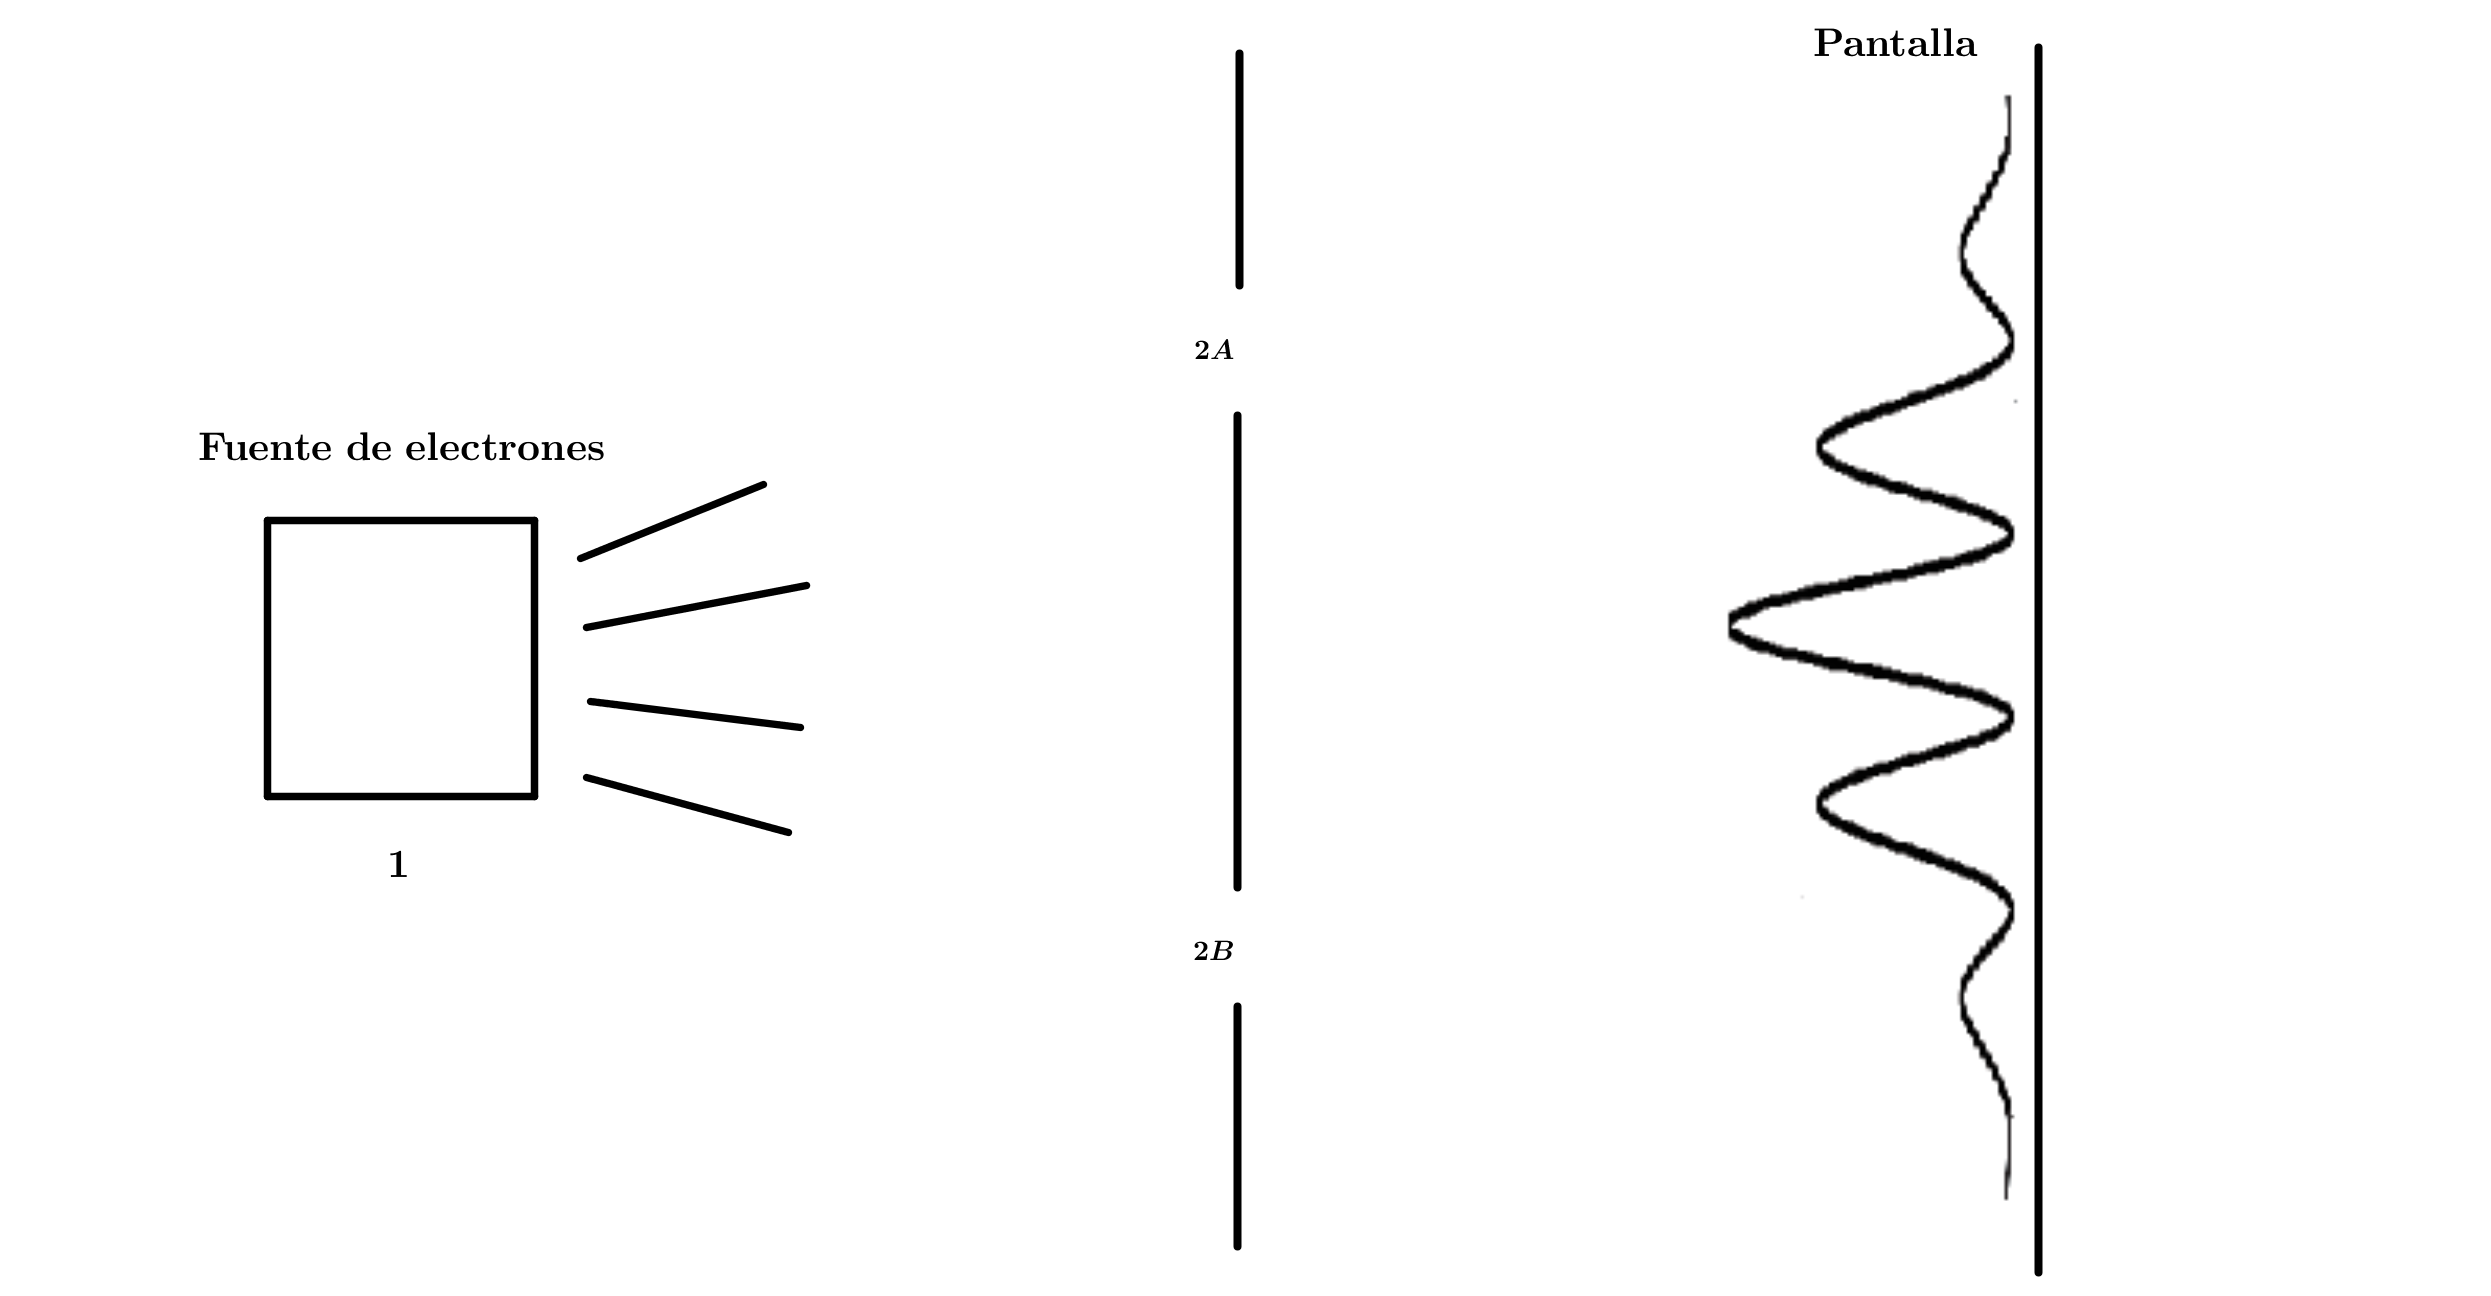
\includegraphics[width=9cm]{Imagenes/Fig1}
\caption[Esquema del experimento de la doble rendija]{Experimento de la doble rendija.}
\end{figure}
si $K(2A,1)$ es la probabilidad de que un electrón pase por la rendija 2A, entonces podemos escribir:
\begin{equation}
K(3,1)=K(2A,1)K(3,2A)+K(2B,1)K(3,2B),
\end{equation}
al tomar el módulo cuadrado de la expresión (2.5) se generarán los términos de interferencia necesarios para describir el patrón de interferencia. No podemos decir que el electrón tomó un camino u el otro, de una manera más simple: este siguió todos los caminos posibles!

\section{La ecuación de Schrödinger.}
En el cuadro de Schrodinger la evolución de un sistema cuántico afecta al ket que representa al estado del sistema [1], la ecuación que rige la dinámica del mismo es la \textbf{Ecuación de Schrödinger}
\begin{equation}
i\hbar\frac{\partial}{\partial t}|\psi\rangle_S=\hat{H}|\psi\rangle_S.
\end{equation}
Sabemos que $\psi(q,t)=\langle q|\psi \rangle_S$ donde $|q\rangle$ son autoestados de la posición, la relacion entre el cuadro de Heisenberg y el de Schrödinger es $|\psi\rangle_H=e^{iHt/\hbar}|\psi\rangle_S$. Si definimos $|qt\rangle \equiv e^{iHt/\hbar}|q\rangle$, entonces $\psi (q,t)=\langle qt|\psi\rangle_H$.

Vamos a mostrar que $K(q_f,t_f;q_i,t_i)=\left\langle q_ft_f|q_it_i \right\rangle$, la relación de completez nos permite escribir:
\begin{eqnarray}
\nonumber \langle q_ft_f|\psi\rangle &=& \int\langle q_ft_f|q_it_i\rangle\langle q_it_i|\psi\rangle dq_i\\
&=& \int \langle q_ft_f|q_it_i\rangle \psi(q_i,t_i)dq_i ,
\end{eqnarray}
y comparando (2.7) y (2.2), vemos que:
\begin{equation}
K(q_f,t_f;q_i,t_i)=\langle q_ft_f|q_it_i\rangle .
\end{equation}
Así, el propagador es proporcional a la amplitud de probabilidad de transición entre el estado inicial $|q_it_i\rangle$ y final $|q_ft_f\rangle$. La idea ahora es expresar el propagador como una integral de trayectoria. Partamos el intervalo temporal $(t_i,t_f)$ en $n+1$ piezas de igual duración $\tau$, así:
\begin{equation}
\langle q_ft_f|q_it_i\rangle = \int dq_1dq_2...dq_n\langle q_ft_f|q_nt_n\rangle \langle q_nt_n|q_{n-1}t_{n-1}\rangle...\langle q_1t_1|q_it_i\rangle .
\end{equation}
Calculemos uno de estos elementos:
\begin{eqnarray}
\nonumber \langle q_{j+1}t_{j+1}|q_jt_j\rangle &=&\langle q_{j+1}|e^{-iHt_{j+1}/\hbar}e^{iHt_j/\hbar}|q_j=\langle q_{j+1}|e^{-i\tau H/\hbar}|q_j\rangle \hspace{0.4cm}\text{A primer orden,}\\
\nonumber &=&\langle q_{j+1}|1-i\tau H/\hbar|q_j\rangle=\delta(q_{j+1}-q_j)-i\tau\hbar\langle q_{j+1}|H|q_j\rangle\\
&=& \frac{1}{2\pi\hbar}\int dp\ \ \exp[\frac{ip}{\hbar}(q_{j+1}-q_j)]-\frac{i\tau}{\hbar}\langle q_{j+1}|H|q_j\rangle , 
\end{eqnarray}	
si asumimos que el Hamiltoniano es una función de $p$ y $q$ de la forma: $H=\frac{p^2}{2m}+V(q)$, entonces:
\begin{eqnarray}
\nonumber \langle q_{j+1}|\frac{p^2}{2m}|q_j \rangle &=& \int dpdp^{\prime} \langle q_{j+1}|p^{\prime}\rangle\langle p^{\prime}|\frac{p^2}{2m}|p\rangle \langle p|q_j \rangle\\
\nonumber &=&\int \frac{dpdp^{\prime}}{2\pi\hbar}\ \ \exp[\frac{i}{\hbar}(p^{\prime} q_{j+1}-pq_j)]\frac{p^2}{2m}\delta(p-p^{\prime})\\
&=& \int \frac{dp}{2\pi\hbar}\ \ \exp[\frac{i}{\hbar}p(q_{j+1}-q_j)]\frac{p^2}{2m} .
\end{eqnarray}
De una manera similar:
\begin{eqnarray}
\nonumber \langle q_{j+1}|V(q)|q_j \rangle &=& V(\frac{q_{j+1}+q_j}{2})\langle q_{j+1}|q_j\rangle\\
\nonumber &=& V(\frac{q_{j+1}+q_j}{2})\delta(q_{j+1}-q_j)\\
\langle q_{j+1}|V(q)|q_j \rangle &=& V(\frac{q_{j+1}+q_j}{2})\int \frac{dp}{2\pi\hbar}\ \ \exp[\frac{i}{\hbar}p(q_{j+1}-q_j)].
\end{eqnarray}
Por tanto $\langle q_{j+1}|H|q_j\rangle=\int \frac{dp}{h}\ \ \exp[\frac{i}{h}p(q_{j+1}-q_j)]H(p,q)$ y :
\begin{equation}
\langle q_{j+1}t_{j+1}|q_jt_j\rangle=\frac{1}{h}\int dp_j\ \ \exp[\frac{i}{\hbar}[p_j(q_{j+1}-q_j)-\tau H(p_j,q_j)]]
\end{equation}
Finalmente:
\begin{equation}
\langle q_{f}t_{f}|q_it_i\rangle=\lim_{N \to \infty}\int\prod_{j=1}^{N}dq_j\prod_{j=0}^{N}\frac{dp_j}{h}\ \ \exp\left\{ \frac{i}{\hbar}\sum_{j=0}^{N}[p_{j}(q_{j+1}-q_{j})-\tau H(p_{j},q_{j})]\right\} ,
\end{equation}
en el continuo:
\begin{equation}
\langle q_{f}t_{f}|q_it_i\rangle=\int\frac{\mathcal{D}q\mathcal{D}p}{h}\ \exp\left\{ \frac{i}{\hbar}\int_{t_{i}}^{t_{f}}(p\dot{q}-H(p,q))dt\right\} . 
\end{equation}
En el continuo $q$ se vuelve una función de $t$ y la integral anterior, es una integral funcional. La expresión (2.15) es la integral de trayectoria para la amplitud de transición entre $(q_i,t_i)$ y $(q_f,t_f)$. Esta integral se hace sobre todas las posibles trayectorias en el espacio de fase y $q(t), p(t)$ son funciones y no operadores, sin embargo es natural preguntarse por la convergencia de (2.15), esto es algo no trivial, sin embargo, de ahora en adelante asumiremos que esta integral existe y converge. 	
\\
Si el Hamiltoniano es tal que $H=\frac{p^2}{2m}+V(q)$
\begin{equation}
\langle q_{f}t_{f}|q_it_i\rangle=\lim_{N \to \infty}\int\prod_{j=1}^{N}dq_j\prod_{j=0}^{N}\frac{dp_j}{h}\ \ \exp\left\{ \frac{i}{\hbar}\sum_{j=0}^{N}[p_{j}(q_{j+1}-q_{j})-\tau \frac{p_j^2}{2m}-V(q)\tau]\right\} ,
\end{equation}
y sabiendo que: $\int_{-\infty}^{\infty}\ \exp[-ax^{2}+bx+c]dx=\ \exp[\frac{b^{2}}{4a}+c](\frac{\pi}{a})^{\frac{1}{2}}$, entonces:
\begin{equation}
\langle q_{f}t_{f}|q_it_i\rangle=\lim_{N\to\infty}[\frac{1}{h}(\frac{\text{\ensuremath{\pi\hbar}2m}}{i\tau})^{\frac{1}{2}}]^{N+1}\int\prod_{1}^{N}dq_{j}\ \exp\left\{ \frac{i}{\hbar}\sum_{0}^{N}\left((\frac{q_{j+1}-q_{j}}{\tau})^{2}\frac{m}{2}-V\right)\tau\right\}. 
\end{equation}
En el continuo:
\begin{equation}
\langle q_{f}t_{f}|q_it_i\rangle=\mathcal{N}\int\mathcal{D}q\ \exp\left\{ \frac{i}{\hbar}\int_{t_{i}}^{t_{f}}\mathcal{L}(q,\dot{q})dt\right\} ,
\end{equation}
donde $\mathcal{L}(q,\dot{q})$ es el lagrangiano clásico, sin embargo, esto solo pasa si asumimos una forma específica del Hamiltoniano, cuando esto no es así se tiene una acción efectiva. En teoría de campos por ejemplo esta descomposición solo se puede hacer en el caso de campos Abelianos.
 
 

\subsection{Teoría de perturbaciones.}

Vamos a ilustrar cómo usar el método de integrales de trayectoria en procesos de dispersión, este tipo de procesos involucran la interacción de una partícula con un potencial $V(x)$. Debido a que no siempre podemos calcular analíticamente la integral (2.18) entonces es necesario acudir a la teoría de perturbaciones, esta es aplicable en el regimen en que la energía de interacción $E_I<\hbar$. En este caso podemos escribir:
\begin{equation}
\ \exp\left[\frac{-i}{\hbar}\int_{t_{i}}^{t_{f}}V(x,t)dt\right]=1-\frac{i}{\hbar}\int_{t_{i}}^{t_{f}}V(x,t)dt+\left(\frac{i}{\hbar}\right)^{2}\frac{1}{2!}\left[\int_{t_{i}}^{t_{f}}V(x,t)dt\right]^{2}+... ,
\end{equation}
cuando reemplazamos esto en la expresión (2.18) obtenemos:
\begin{equation}
K=K_0+K_1+K_2+...\ \text{donde}\ K_0=\mathcal{N}\int \mathcal{D}x \ \exp\left[ \frac{i}{\hbar}\int \frac{1}{2}m\dot{x}^2dt\right] .
\end{equation}
Para calcular $K_0$, escribamos la forma discretizada de (2.20)
\begin{eqnarray}
\nonumber K_0&=&\lim_{n\to\infty}\left(\frac{m}{i\hbar\tau}\right)^{\left(\frac{n+1}{2}\right)}\int_{-\infty}^{\text{\ensuremath{\infty}}}\prod_{j=1}^{n}dx_{j}\ \exp\left[\frac{im}{2\hbar\tau}\sum_{j=0}^{n}\left(x_{j+1}-x_{j}\right)^{2}\right]\\
\nonumber &=& \lim_{n\to\infty}\left(\frac{m}{i\hbar\tau}\right)^{\left(\frac{n+1}{2}\right)}\frac{1}{\left(n+1\right)^{\frac{1}{2}}}\left(\frac{i\hbar\tau}{m}\right)^{\frac{n}{2}}\ \exp\left[\frac{im}{2\hbar(n+1)\tau}\left(x_{f}-x_{i}\right)^{2}\right]\\
K_0(x_ft_f,x_it_i)&=& \Theta(t_{f}-t_{i})\left(\frac{m}{i\hbar(t_{f}-t_{i})}\right)^{1/2}\ \exp\left[\frac{im}{2\hbar(t_{f}-t_{i})}\left(x_{f}-x_{i}\right)^{2}\right] .
\end{eqnarray}
Calculemos ahora $K_1$:
\begin{equation}
K_1=\lim_{n\to\infty}\frac{-i}{\hbar}N^{(n+1)/2}\sum_{i=1}^{n}\int\ \exp\left[\frac{im}{2\hbar\tau}\sum_{j=0}^{n}(x_{j+1}-x_{j})^{2}\right]V(x_{i},t_{i})dx_{1}...dx_{n}.
\end{equation}
Ahora como solo $V(x)$ depende de $x_i$, separamos (2.22) como:
\begin{eqnarray}
\nonumber K_1&=&\lim_{n\to\infty}\frac{-i}{\hbar}\sum_{i=1}^{n}\left\{ \int N^{(n-i+1)/2}\ \exp\left[\frac{im}{2\hbar\tau}\sum_{j=i}^{n}(x_{j+1}-x_{j})^{2}\right]dx_{i}...dx_{n}\right\}\\
& &\times  \left\{ \int N^{i/2}\ \exp\left[\frac{im}{2\hbar\tau}\sum_{j=0}^{i-1}(x_{j+1}-x_{j})^{2}\right]dx_{1}...dx_{i-1}\right\} V(x_{i},t_{i}),
\end{eqnarray}
los dos términos en corchetes en (2.23) son $K_0(xt,x_ft_f)$ y $K_0(x_it_i,xt)$, así:
\begin{equation}
K_1(x_ft_f,x_it_i)= -\frac{i}{\hbar}\int_{t_{i}}^{t_{f}}dt\int_{-\infty}^{\infty}K_{0}(x_{f}t_{f}.xt)V(x,t)K_{0}(xt,x_{i}t_{i})dx .
\end{equation}
Como $K_0(x_ft_f,xt)=0$ si $t>t_f$ y $K_0(xt,x_it_i)=0$ si $t<t_i$, entonces podemos escribir:
\begin{equation}
K_1(x_ft_f,x_it_i)=-\frac{i}{\hbar}\int_{-\infty}^{\infty}dt\int_{-\infty}^{\infty}K_{0}(x_{f}t_{f}.xt)V(x,t)K_{0}(xt,x_{i}t_{i})dx .
\end{equation}
De la misma manera se puede probar que:
\begin{equation}
K_2(x_ft_f,x_it_i)=\left(\frac{-i}{\hbar}\right)^2\int_{-\infty}^{\infty}dt_{1}dt_{2}dx_{1}dx_{2}K_{0}(x_{f}t_{f}.x_{2}t_{2})V_2K_{0}(x_{2}t_{2},x_{1}t_{1})V_1K_{0}(x_{1}t_{1},x_{i}t_{i}).
\end{equation}
Esta es una solución en series para $K$ y recibe el nombre de Serie de Born, en la expresión general para $K_n$ no se tiene el factor $n!$ ya que hay ese mismo numero de formas para ordenar los $n$ potenciales $V(x)$ que entran en el propagador.
\\
\\
Por último mostraremos que \textbf{el propagador es la función de Green de la ecuación de Schrödinger.} Para esto sustituyamos la expresión para la serie de Born en la ecuación (2.2):
\begin{eqnarray}
\nonumber \psi(\vec{x}_f,t_f)&=&\int K_{0}(\vec{x_{f}}t_{f},\vec{x_{i}}t_{i})\psi(\vec{x_{i}},t_{i})d\vec{x_{i}}\\
& & \frac{-i}{\hbar}\int K_{0}(\vec{x_{f}}t_{f},\vec{x}t)V(\vec{x},t)K_{0}(\vec{x}t,\vec{x_{i}}t_{i})\psi(\vec{x_{i}},t_{i})d\vec{x}dtd\vec{x_{i}}+O(\hbar^{2}),
\end{eqnarray}
hemos cambiado a tres dimensiones espaciales y los otros términos en la serie hacen converger el último $K_0$ a $K$, por tanto:
\begin{equation}
\psi(\vec{x}_f,t_f)=\int K_{0}(\vec{x_{f}}t_{f},\vec{x_{i}}t_{i})\psi(\vec{x_{i}},t_{i})d\vec{x_{i}}-\frac{i}{\hbar}\int K_{0}(\vec{x_{f}}t_{f},\vec{x}t)V(\vec{x},t)\psi(\vec{x},t)d\vec{x}dt .
\end{equation}
Cuando $t_i \to -\infty$,no hay presencia de potencial por tanto $\psi$ se vuelve una onda plana. Así:
\begin{equation}
\psi(\vec{x}_f,t_f)=\phi(\vec{x}_ft_f)-\frac{i}{\hbar}\int K_{0}(\vec{x_{f}}t_{f},\vec{x}t)V(\vec{x},t)\psi(\vec{x},t)d\vec{x}dt.
\end{equation}
Aplicando el operador $\hat{H}=\frac{\hbar^2}{2m}\nabla_{\vec{x}_ft_f}+i\hbar\frac{\partial}{\partial t_f}$ en la ecuación (donde $\nabla_{\vec{x}_ft_f}$ denota diferenciación respecto a $\vec{x}_ft_f$ )(2.29) y usando $\hat{H}\psi(x,t)=V(x,t)\psi(x,t)$:
\begin{eqnarray}
\nonumber \hat{H}(\psi(\vec{x}_f,t_f))&=&\hat{H}(\phi(\vec{x}_ft_f))-\frac{i}{\hbar}\int\hat{H} (K_{0}(\vec{x_{f}}t_{f},\vec{x}t))V(\vec{x},t)\psi(\vec{x},t)d\vec{x}dt\\
\nonumber V(\vec{x}_f,t_t)\psi(\vec{x}_f,t_f)&=&0-\frac{i}{\hbar}\int\hat{H} (K_{0}(\vec{x_{f}}t_{f},\vec{x}t))V(\vec{x},t)\psi(\vec{x},t)d\vec{x}dt ,
\end{eqnarray}
por tanto:
\begin{equation}
\left(\frac{\hbar^2}{2m}\nabla_{\vec{x}_ft_f}+i\hbar\frac{\partial}{\partial t_f}\right)K_{0}(\vec{x_{f}}t_{f},\vec{x}t)=i\hbar\delta(\vec{x}-\vec{x}_f)\delta(t-t_f).
\end{equation}
Esto último era lo que queríamos probar.








\subsection{Matriz $\mathcal{S}$.}
En un experimento de dispersión es razonable suponer que las partículas al principio y al final del proceso son partículas libres, estas ondas planas están distribuidas en todo el espacio. Sin embargo, esto último lleva a una contradicción ya que la presencia del centro dispersor no permite que en sus cercanias la solución sea una onda plana. Para resolver este inconveniente se puede proponer lo que se llama una fuente dinámica, que se "prenda y apague" lentamente tal que las partículas en los estados (final/incial) puedan ser libres y por tanto la aproximación de ondas planas sea válida en este regimen.\\
\\
Para empezar definamos $\psi_{in}(\vec{x}_i,t_i)$, $\psi_{out}(\vec{x}_f,t_f)$ como ondas planas para $t\to -\infty$,  $t\to \infty$ respectivamente, la amplitud de dispersión se define como:
\begin{equation}
\mathcal{S}=\int\psi_{out}^{*}(\vec{x}_{f}t_{f})\psi^{(+)}(\vec{x}_{f}t_{f})d\vec{x}_{f}.
\end{equation}
En (2.31) el superíndice $(+)$ denota que $\psi^{(+)}(\vec{x}t)$ era una onda libre en $t\to -\infty$, usando la serie de Born obtenemos:
\begin{eqnarray}
\nonumber \mathcal{S}&=&\int\psi_{out}^{*}(\vec{x}_{f}t_{f})\psi^{(+)}(\vec{x}_{f}t_{f})d\vec{x}_{f}=\int\psi_{out}^{*}(\vec{x}_{f}t_{f})K_{0}(\vec{x}_{f}t_{f},\vec{x}_{i}t_{i})\psi_{in}(\vec{x}_{i}t_{i})d\vec{x}_{f}d\vec{x_{i}}\\
\nonumber &&-\frac{i}{\hbar}\int\psi_{out}^{*}(\vec{x}_{f}t_{f})K_{0}(\vec{x}_{f}t_{f},\vec{x}t)V(\vec{x}t)K_{0}(\vec{x}t,\vec{x}_{i}t_{i})\psi_{in}(\vec{x}_{i}t_{i})d\vec{x}_{f}d\vec{x_{i}}d\vec{x}dt\\
\nonumber &=&\int \psi_{out}^{*}(\vec{x}_{f}t_{f})\phi(\vec{x}_{f}t_{f})d\vec{x}_f\\
&&-\frac{i}{\hbar}\int\psi_{out}^{*}(\vec{x}_{f}t_{f})K_{0}(\vec{x}_{f}t_{f},\vec{x}t)V(\vec{x}t)K_{0}(\vec{x}t,\vec{x}_{i}t_{i})\psi_{in}(\vec{x}_{i}t_{i})d\vec{x}_{f}d\vec{x_{i}}d\vec{x}dt.   
\end{eqnarray}
Si los momentos iniciales y finales son $\vec{p}_i=\hbar\vec{k}_i$,$\vec{p}_f=\hbar\vec{k}_f$ respectivamente, entonces tenemos que:
\begin{eqnarray}
\psi_{in}(\vec{x}t)&=&\frac{1}{\sqrt{\tau}}\ \exp\left( \frac{i}{\hbar}(\vec{p}_i\cdot \vec{x}-E_it )\right)\\
\psi_{out}(\vec{x}t)&=&\frac{1}{\sqrt{\tau}}\ \exp\left( \frac{i}{\hbar}(\vec{p}_f\cdot \vec{x}-E_ft )\right),
\end{eqnarray}
donde $E^2=\frac{p^2}{2m}$ y $\tau$ es el volumen de integración, el cual es arbitrario. Si sustituimos las expresiones (2.33) y (2.34) en (2.32) obtenemos:
\begin{equation}
\mathcal{S}_{fi}=\delta(\vec{k}_f-\vec{k}_i)-\frac{i}{\hbar}\int\psi_{out}^{*}(\vec{x}_{f}t_{f})K_{0}(\vec{x}_{f}t_{f},\vec{x}t)V(\vec{x}t)K_{0}(\vec{x}t,\vec{x}_{i}t_{i})\psi_{in}(\vec{x}_{i}t_{i})d\vec{x}_{f}d\vec{x_{i}}d\vec{x}dt.
\end{equation}
Lo cual nos permite ver la amplitud de dispersion $\mathcal{S}_{fi}$ como el elemento de una matriz, la \textbf{matriz $\mathcal{S}$ de dispersión}. En (2.35) el primer término solo es representativo cuando no hay interacción y $\vec{k}_i=\vec{k}_f$. Las interacciones están representadas en el segundo término.\\
\\
Es posible representar este segundo término mediante una serie de diagramas a los cuales se les asocian ciertas reglas, estos diagramas reciben el nombre de \textbf{Diagramas de Feynmann}. Si nombramos:
\begin{equation}
\mathcal{A}=-\frac{i}{\hbar}\int\psi_{out}^{*}(\vec{x}_{f}t_{f})K_{0}(\vec{x}_{f}t_{f},\vec{x}t)V(\vec{x}t)K_{0}(\vec{x}t,\vec{x}_{i}t_{i})\psi_{in}(\vec{x}_{i}t_{i})d\vec{x}_{f}d\vec{x_{i}}d\vec{x}dt,
\end{equation}

\begin{SCfigure}[1.3][h]
\caption[Diagrama de Feynmann primera cuantización]{Representación de $\mathcal{A}$.}
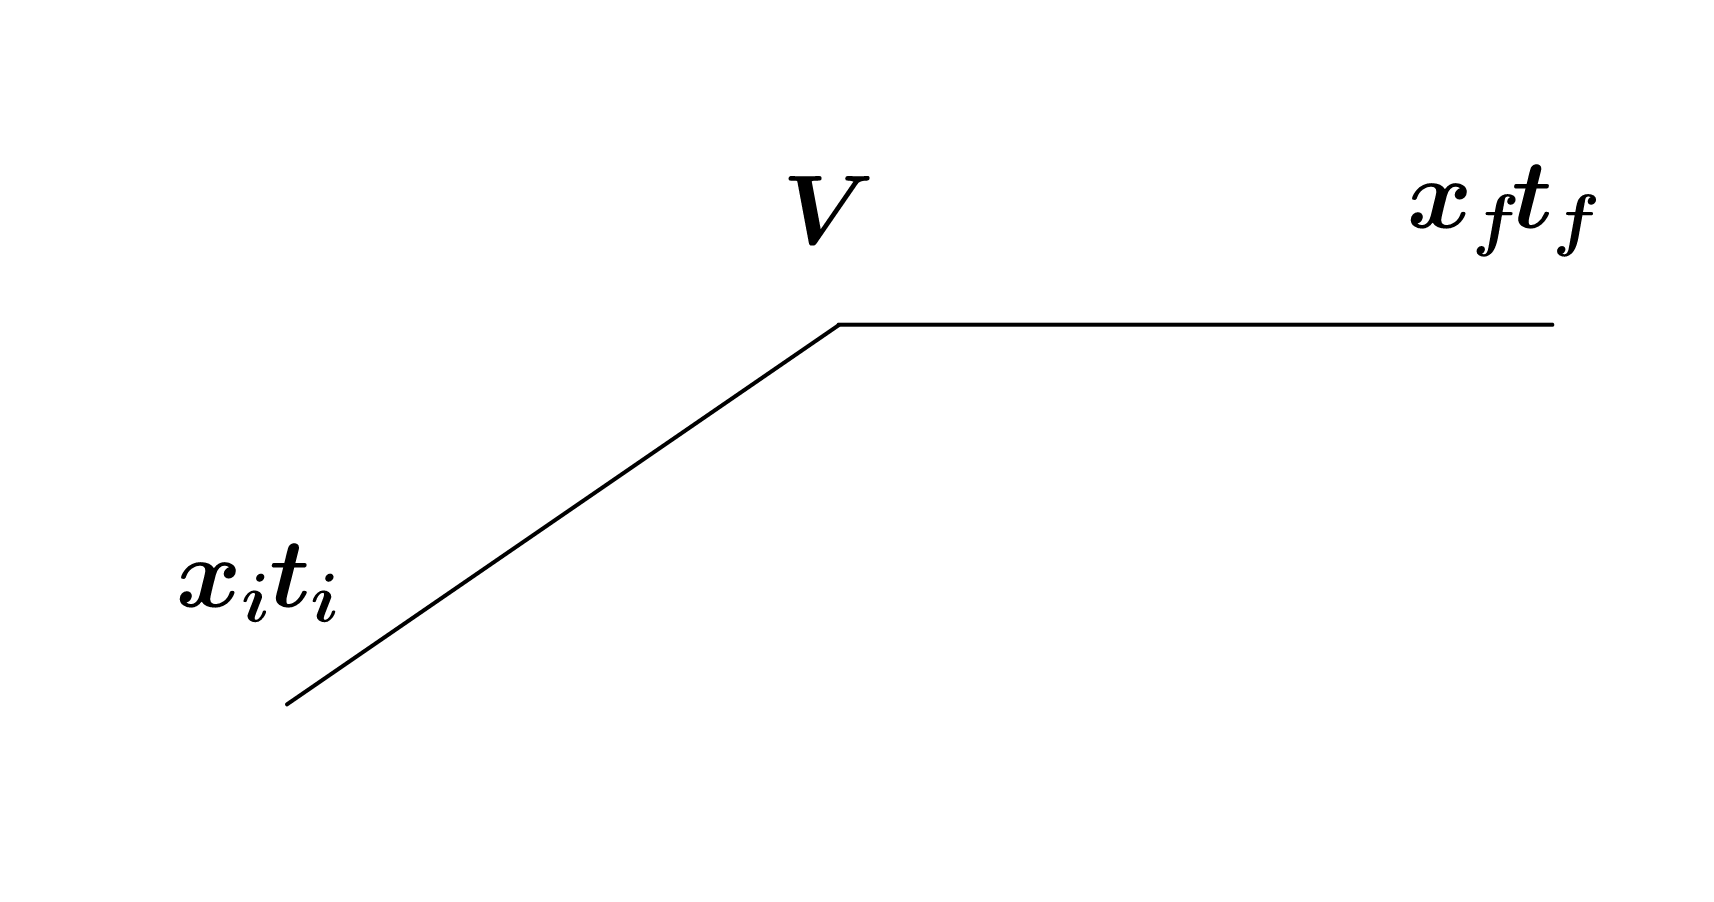
\includegraphics[width=4cm]{Imagenes/Fig2}
\end{SCfigure}
este diagrama lo podemos descomponer usando la siguiente convención:
\begin{SCfigure}[1.3][h]
\caption[Diagrama de Feynmann primera cuantización]{Representación de $K_0(x_2t_2,x_1t_1)$.}
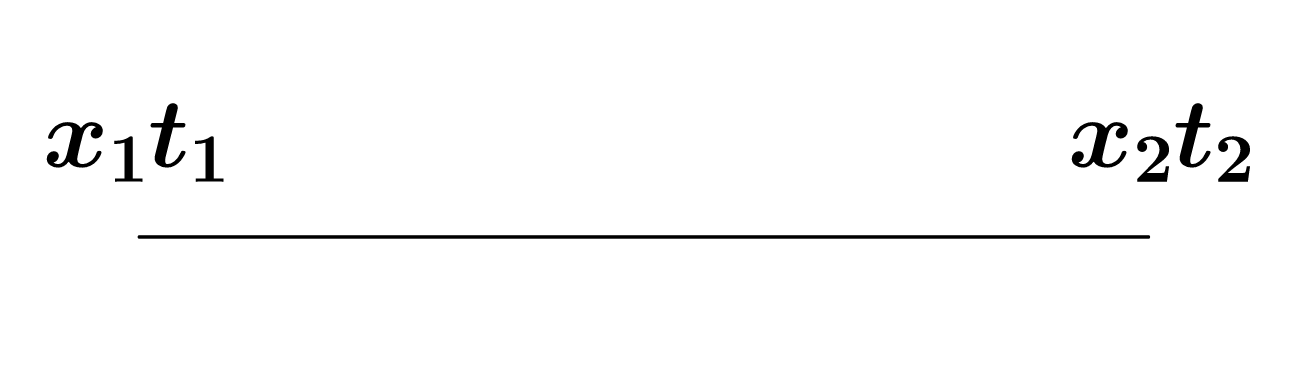
\includegraphics[width=4cm]{Imagenes/Fig3}
\end{SCfigure}
\begin{SCfigure}[1.3][h]
\caption[Diagrama de Feynmann primera cuantización]{Representación de $\int -\frac{i}{\hbar}V(xt)dxdt$.}
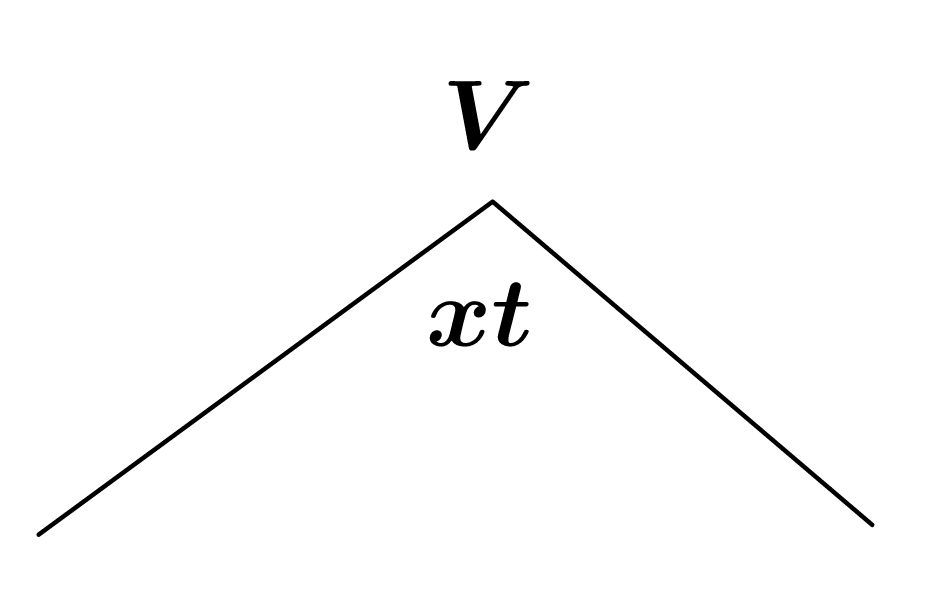
\includegraphics[width=4cm]{Imagenes/Fig4}
\end{SCfigure}
\\
Por ejemplo el diagrama correspondiente a término de segundo orden:
\begin{eqnarray}
\nonumber \mathcal{A}^{(2)}&=&\left(-\frac{i}{\hbar}\right)^2\int d\vec{x}_{f}d\vec{x_{i}}d\vec{x^{\prime}}dt^{\prime} d\vec{x}dtK_{0}(\vec{x}t,\vec{x}_it_i)V(\vec{x}t)K_{0}(\vec{x}^{\prime} t^{\prime},\vec{x}t)\\
&&\times V(\vec{x}^{\prime} t^{\prime})K_{0}(\vec{x}_{f}t_{f},\vec{x}^{\prime} t^{\prime})\psi_{out}^{*}(\vec{x}_{f}t_{f})\psi_{in}(\vec{x}_{i}t_{i}),
\end{eqnarray}
es el que se muestra enm la figura 2.5 .
\begin{SCfigure}[1.3][h]
\caption[Diagrama de Feynmann primera cuantización]{Representación de $\mathcal{A}^{(2)}$}
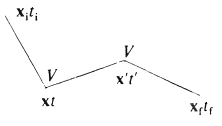
\includegraphics[width=4cm]{Imagenes/Fig5}
\end{SCfigure}
\\
\\
En algunos casos es útil conocer una expresión para el propagador  $K_0$ en el espacio de momentos, definimos $\mathcal{K}_0(\vec{p}_1t_1,\vec{p}_2t_2)$ como la amplitud de que una partícula con momento $\vec{p}_2$ en un instante $t_2$, sea observada un instante de tiempo después en $t_1$ con momento $\vec{p}_1$. Así:
\begin{eqnarray}
\nonumber \mathcal{K}_0(\vec{p}_1t_1,\vec{p}_0t_0)&=&\int \ \exp\left(\frac{-i}{\hbar}(\vec{p}_1\cdot\vec{x}_1)\right) K_0(\vec{x}_1t_1,\vec{x}_0t_0)\ \exp\left(\frac{-i}{\hbar}(\vec{p}_0\cdot\vec{x}_0)\right)d\vec{x}_0d\vec{x}_1\\
&&\nonumber \Theta(t_{1}-t_{0})\left(\frac{m}{i\hbar(t_{1}-t_{0})}\right)^{1/2}\int\ \exp\left[\frac{i}{\hbar}(\vec{p}_{0}\cdot\vec{x}_{0}-\vec{p}_{1}\cdot\vec{x}_{1})\right]\\
&& \times \ \exp\left[\frac{im(\vec{x}_{0}-\vec{x}_{1})^{2}}{2\hbar(t_{1}-t_{0})}\right]d\vec{x}_{0}d\vec{x}_{1},
\end{eqnarray}
ahora si introducimos las siguientes variables:
\begin{equation}
\vec{x}=\vec{x}_0-\vec{x}_1;\hspace{0.3cm}\vec{X}=\vec{x}_0+\vec{x}_1;\hspace{0.3cm}\vec{p}=\vec{p}_0-\vec{p}_1;\hspace{0.3cm}\vec{P}=\vec{p}_0+\vec{p}_1 ,
\end{equation}
teniendo en cuenta que el Jacobiano de esta transformación es $J=\left(\frac{1}{2}\right)^3=\frac{1}{8}$ y con $\alpha=\frac{m}{2\hbar (t_1-t_0)}$  podemos escribir:
\begin{equation}
\mathcal{K}_0(\vec{p}_1t_1,\vec{p}_0t_0)=\Theta(t_{1}-t_{0})\left(\frac{\alpha}{i\pi}\right)^{3/2}\frac{1}{8}\int\ \exp\left[\frac{i\vec{p}\cdot\vec{X}}{2\hbar}\right]d\vec{X}\int\ \exp\left[\frac{i\vec{P}\cdot\vec{x}}{2\hbar)}\right]e^{i\alpha x^{2}}d\vec{x}.
\end{equation}
La primera integral es $I_1=8(2\pi\hbar)^3\delta(\vec{p}_0-\vec{p}_1)$, la segunda la podemos calcular con la identidad $ \int e^{-ax^2+bx+c}=e^{\frac{b^2}{4a}+c}\left(\frac{\pi}{a}\right)^(1/2)$, por tanto $I_2=\left(\frac{i\pi}{\alpha}\right)^{3/2}\ \exp\left[\frac{-i\vec{P}^{2}}{8\hbar^{3}4i\alpha}\right]$, por tanto:
\begin{equation}
\mathcal{K}_0(\vec{p}_1t_1,\vec{p}_0t_0)=(2\pi\hbar)^3\Theta(t_1-t_0)\delta(\vec{p}_1-\vec{p}_0)\ \exp\left[\frac{-i\vec{P}^{2}(t_{1}-t_{0})}{8m\hbar}\right].
\end{equation}
Si también realizamos la transformada de Fourier en el tiempo, obtenemos:
\begin{equation}
\mathcal{K}_0(\vec{p}_1E_1,\vec{p}_0E_0)=(2\pi\hbar)^4\delta(\vec{p}_0-\vec{p}_1)\delta(E_1-E_0)\frac{i\hbar}{E-\frac{p_{1}^{2}}{2m}+i\epsilon}.
\end{equation}
De lo anterior las reglas de Feynmann en el espacio de momentos son:
\begin{SCfigure}[1.3][h]
\caption[Diagrama de Feynmann primera cuantización]{Representación de $\frac{1}{(2\pi\hbar)^4}\frac{i\hbar}{E-\frac{p_{1}^{2}}{2m}+i\epsilon}$}
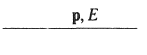
\includegraphics[width=4cm]{Imagenes/Fig6}
\end{SCfigure}
\begin{SCfigure}[1.3][h]
\caption[Diagrama de Feynmann primera cuantización]{Representación de $\frac{-i}{\hbar}(2\pi\hbar)^4v(\vec{q},W)$}
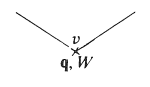
\includegraphics[width=4cm]{Imagenes/Fig7}
\end{SCfigure}

\subsection{Propiedades adicionales de las integrales de trayectoria.}
Ya hemos mostrado que la amplitud de transición entre un estado $(q_i,t_i)$ a $(q_f,t_f)$ está dada por:
\begin{equation}
\langle q_{f}t_{f}|q_it_i\rangle=\mathcal{N}\int\mathcal{D}q\text{Exp\ensuremath{\left\{ \frac{i}{\hbar}\int_{t_{i}}^{t_{f}}\mathcal{L}(q,\dot{q})dt\right\} }}.
\end{equation}
En un experimento real, las partículas creadas en algún instante en el pasado son destruidas al ser detectadas, esto lo podemos interpretar de la siguiente manera: El estado de vacío en $t=-\infty$ evoluciona al mismo vacío en $t=\infty$. En este proceso una partícula es creada para ser posteriormente destruida, todo esto en presencia de una fuente generadora de estos procesos. Así es razonable poner nuestro interés en calcular transiciones vacío-vacío en presencia de una fuente.\\
\\
Podemos modificar el Lagrangiano de la de la siguiente manera: $\mathcal{L} \to \mathcal{L}+\hbar J(t)q(t)$. Si $|0,t\rangle^J $ es el estado fundamental en presencia de la fuente, entonces la amplitud de transición se define de la siguiente manera:
\begin{equation}
Z[J]\propto \langle 0,\infty|0,-\infty\rangle ^J.
\end{equation}
La fuente $J(t)=0$ para $t>t^{\prime}$ , $t^{\prime} < t$. Instroduzcamos entonces $T$ y $T^{\prime} $ de tal manera que $T<t^{\prime} $ , $T^{\prime}>t^{\prime} $ por tanto la amplitud (2.44) es:
\begin{equation}
\langle 	Q^{\prime} T^{\prime} |QT\rangle=\mathcal{N}\int\mathcal{D}q\text{Exp\ensuremath{\left\{ \frac{i}{\hbar}\int_{T}^{T^{\prime}}\mathcal{L}(q,\dot{q})dt\right\} }},
\end{equation}
podemos escribir:
\begin{equation}
\langle Q^{\prime} T^{\prime} |QT \rangle^J=\int dq^{\prime} dq\langle Q^{\prime} T^{\prime} | q^{\prime} t^{\prime}  \rangle\langle q^{\prime} t^{\prime} | qt \rangle\langle qt|QT \rangle .
\end{equation}
Ahora si denotamos $|E_q\rangle$ como un autoestado del hamiltoniano podemos usar estos estados para expandir:
\begin{eqnarray}
\nonumber \langle Q^{\prime} T^{\prime} | q^{\prime} t^{\prime}  \rangle &=& \langle Q\prime|\ \exp\left[\frac{-i}{\hbar}HT^{\prime}\right]\ \exp\left[\frac{i}{\hbar}Ht^{\prime}\right]|q^{\prime}\rangle\\
\nonumber &=& \sum_{mn}\phi^{*}(q^{\prime})\phi(Q^{\prime})\langle E_{Q^{\prime}}|\ \exp\left[\frac{-i}{\hbar}HT^{\prime}\right]\ \exp\left[\frac{i}{\hbar}Ht^{\prime}\right]|E_{q^{\prime}}\rangle\\
&=&\sum_{m}\phi^{*}(q^{\prime})\phi(Q^{\prime}) \exp\left[\frac{i}{\hbar}E_{m}(t^{\prime}-T^{\prime})\right],
\end{eqnarray}
de la misma manera:
\begin{equation}
\langle qt|	QT  \rangle=\sum_{m}\phi^{*}(Q)\phi(q)\ \exp\left[\frac{i}{\hbar}E_{m}(t-T)\right].
\end{equation}
Introduciendo (2.47) y (2.48) en (2.46):
\begin{eqnarray}
\nonumber \langle Q^{\prime} T^{\prime}|QT\rangle &=&\int dq^{\prime} dq\sum_{m}\phi_{m}(Q^{\prime})\phi_{m}(q^{\prime},t)\ \exp\left[\frac{-i}{\hbar}E_{m}T^{\prime}\right]\\
&&\times  \sum_{n}\phi_{n}^{*}(Q)\phi_{n}^{*}(q,t)\ \exp\left[\frac{i}{\hbar}E_{n}T\right]\langle q^{\prime} t^{\prime}|qt\rangle^{J}.
\end{eqnarray}
Si hacemos una rotación de Wick de $T$ y $T^{\prime} $ nos damos cuenta que el término que menos sufre de supresión en la integral (2.49) es el asociado a $m=n=0$, por tanto:
\begin{equation}
\int dq^{\prime} dq\phi_{0}^{*}(q^{\prime},t^{\prime})\langle q^{\prime} t^{\prime}|qt\rangle^{J}\phi_{0}(q,t)=\lim_{T\to-\text{\ensuremath{\infty}e}^{-i\delta},T^{\prime}\to\text{\ensuremath{\infty}e}^{-i\delta}}\frac{\langle Q^{\prime} T^{\prime}|QT\rangle^{J}}{\phi_{0}^{*}(Q)\phi_{0}(Q^{\prime})\ \exp\left[\frac{-i}{\hbar}E_{0}(T^{\prime}-T)\right]}.
\end{equation}
El RHS de (2.50) es simplemente el valor de expectación en el vacio de la amplitud de transcición, justo lo que buscabamos y el denominador de la parte derecha de la ecuación es simplemente una constante, así:
\begin{equation}
\langle 0,\infty| 0,-\infty \rangle ^J \propto \lim_{T\to-\text{\ensuremath{\infty}e}^{-i\delta},T^{\prime}\to\text{\ensuremath{\infty}e}^{-i\delta}}\langle Q^{\prime} T^{\prime}|QT\rangle^{J}.
\end{equation}
Otra forma equivalente de obtener este mismo resultado es: en vez de hacer una rotación de Wick, podemos agregar una pequeña cantidad imaginaria negativa al hamiltoniano $H+(-\frac{1}{2}i\epsilon q^2)$, lo cual es equivalente a restar esta misma cantidad a $\mathcal{L}$, de aquí que:
\begin{equation}
Z[J]=\int\mathcal{D}q\ \exp\left\{ \frac{i}{\hbar}\int_{-\infty}^{\infty}(\mathcal{L}(q,\dot{q})+\hbar Jq + \frac{1}{2}i\epsilon q^2)dt\right\} .
\end{equation}
En general se cumple que:
\begin{equation}
 \langle q_{f}t_{f}|T[q(t_{1})...q(t_{n})]|q_{i}t_{i}\rangle=\mathcal{N}\int\mathcal{D}qq(t_{1})...q(t_{n})\ \exp\left[\frac{i}{\hbar}\int_{t_{i}}^{t_{f}}\mathcal{L}dt\right],
\end{equation}
donde $T$ es el operador de ordenamiento temporal. Si derivamos funcionalmente la expresión para $Z[J]$ respecto a $J(t)$ obtenemos:
\begin{equation}
\frac{\delta Z[J]}{\delta J(t_{1}).}|_{J=0}=i\mathcal{N}\int\mathcal{D}qq(t_{1})\ \exp\left[\frac{i}{\hbar}\int_{t_{i}}^{t_{f}}\mathcal{L}dt\right],
\end{equation}	
haciendo esto $n$ veces:
\begin{equation}
\frac{\delta^{n}Z[J]}{\delta J(t_{1})...\delta J(t_{n}).}|_{J=0}=i^{n}\mathcal{N}\int\mathcal{D}qq(t_{1})...q(t_{n})\ \exp\left[\frac{i}{\hbar}\int_{t_{i}}^{t_{f}}\mathcal{L}dt\right].
\end{equation}
De igualar las ecuaciones (2.53), (2.55) y al tener en cuenta agregar el factor $\frac{1}{2}i\epsilon q^2$ (el cual simplemente va a hacer converger los estados inicial y final en (2.53) a estados de vacío) obtenemos:
\begin{equation}
\frac{\delta^{n}Z[J]}{\delta J(t_{1})...\delta J(t_{n}).}|_{J=0}\propto i^{n}\langle0,\infty|T[q(t_{1})...q(t_{n})]|0,-\infty\rangle .
\end{equation}
Estas últimas expresiones que hemos derivado van a ser importantes como punto de partida a la hora de tratar de cuantizar una teoría de campos vía el formalismo de integrales de trayectoria.
\newpage


\section{El experimento de la doble rendija.}
En esta sección aplicaremos lo aprendido en la $\mathsection$2.1 para resolver vía integrales de trayectoria el conocido problema de la difracción de electrones por una y dos rendijas. 

\subsection{El propagador de una partícula libre.}

Con este objetivo en mente primero necesitamos conocer el propagador de una partícula libre, sabemos que en un espacio plano de una dimensión la integral de trayectoria está dada por la expresión (2.17),podemos hacer fácilmente una analogía para un espacio euclídeo d-dimensional. En este caso el propagador es:
\begin{eqnarray}
\nonumber K(x_{f}t_{f,},x_{i,}t_{i})&=&\lim_{n\to\infty}\frac{1}{(2\pi i\hbar\epsilon/m)^{d/2}}\prod_{k=1}^{n}\int\frac{d^{d}x_{k}}{(2\pi i\hbar\epsilon/m)^{d/2}}\\
&&\times \ \exp\left\{ \frac{i}{\hbar}\sum_{k=1}^{n}\epsilon\left[\frac{m(x_{k}-x_{k-1})^{2}}{2\epsilon^{2}}-V(x_{k})\right]\right\}, 
\end{eqnarray}
donde $\epsilon=(t_i-t_f)/n$; para una partícula libre $V(x_k)=0$, entonces:
\begin{equation}
K(x_{f}t_{f,},x_{i,}t_{i})=\lim_{n\to\infty}\frac{1}{(2\pi i\hbar\epsilon/m)^{d/2}}\prod_{k=1}^{n}\int\frac{d^{d}x_{k}}{(2\pi i\hbar\epsilon/m)^{d/2}}\ \exp\left\{ \frac{i}{\hbar}\sum_{k=1}^{n}\left[\frac{m(x_{k}-x_{k-1})^{2}}{2\epsilon}\right]\right\}.
\end{equation}
Para $d=1$, integremos los términos que tienen que ver con $x_1$:
\begin{eqnarray}
\nonumber &\frac{1}{(2\pi i\hbar\epsilon/m)^{1/2}}\prod_{k=1}^{n}\int\frac{dx_{1}}{(2\pi i\hbar\epsilon/m)^{1/2}}\ \exp\left\{ \frac{im(x_{1}-x_{0})^{2}}{2\hbar\epsilon}\right\} \ \exp\left\{ \frac{im(x_{2}-x_{1})^{2}}{2\hbar\epsilon}\right\}\\
\nonumber &=\frac{1}{(2\pi i\hbar\epsilon/m)}\int dx_{1}\ \exp\left\{ \frac{-m}{2i\epsilon\hbar}\left(2x_{1}^{2}-2x_{1}(x_{2}+x_{0})+x_{0}^{2}+x_{2}^{2}\right)\right\}\\
\nonumber &\text{Usando} \ \int e^{-ax^{2}+bx+c}dx=e^{^{\frac{b^{2}}{4a}+c}}\left(\frac{\pi}{a}\right)^{1/2}\\
\nonumber &=\frac{1}{\sqrt{2\pi i\hbar(2\epsilon)/m}}\ \exp\left\{ \frac{im(x_{2}-x_{0})^{2}}{2\hbar(2\epsilon)}\right\}, 
\end{eqnarray}
ahora al seguir con la integral de $x_2$ queda:
\begin{eqnarray}
\nonumber & \frac{1}{(2\pi i\hbar\epsilon/m)\sqrt{2}}\int dx_{2}\ \exp\left\{ \frac{im}{2\hbar(2\epsilon)}\left(x_{2}-x_{o}\right)^{2}\right\} \ \exp\left\{ \frac{im}{2\hbar\epsilon}\left(x_{3}-x_{2}\right)^{2}\right\} \\
&=\frac{1}{\sqrt{2\pi i\hbar(3\epsilon)/m}}\ \exp\left\{ \frac{im(x_{3}-x_{0})^{2}}{2\hbar(3\epsilon)}\right\}. 
\end{eqnarray}
Así, por inducción:
\begin{eqnarray}
\nonumber K(x_{f}t_{f},x_{i}t_{i})&=&\lim_{n\to\infty}\frac{1}{\sqrt{2\pi i\hbar(n\epsilon)/m}}\ \exp\left\{ \frac{im(x_{f}-x_{i})^{2}}{2\hbar(n\epsilon)}\right\} \\
&=& \frac{1}{\sqrt{2\pi i\hbar(t_{f}-t_{i})/m}}\ \exp\left\{ \frac{im(x_{f}-x_{i})^{2}}{2\hbar(t_{f}-t_{i})}\right\} .
\end{eqnarray}
Por tanto en 3-D:
\begin{equation}
K^{3D}(x_{f}t_{f},x_{i}t_{i})\equiv K_{0}^{3D}=\left(\frac{m}{2\pi i\hbar(t_{f}-t_{i})}\right)^{3/2}\ \exp\left\{ \frac{im|\vec{x}_{f}-\vec{x}_{i}|^{2}}{2\hbar(t_{f}-t_{i})}\right\} .
\end{equation}


\subsection{El problema de difracción e interferencia.}
Consideremos el siguiente experimento: una fuente de electrones en $(x,y,z)=(0,0,0)$ y dos rendijas en $Z=D$ con ancho $2a$ y centradas en $x=\pm b$, tal como se muestra en la figura 2.6. Adicionalmente consideramos que las barreras son lo suficientemente largas en $y$ como para poder despreciar los efectos de difracción inducidos en el caso de que estas fueran finitas.\\
\\
Así reducimos la dimensión del propagador en $y$:
\begin{eqnarray}
\nonumber K_{0}^{2D}(\vec{r}t,\vec{r}^{\prime} t^{\prime})&=&\int_{-\infty}^{\infty}dyK_{0}^{3D}(\vec{r}t,\vec{r}^{\prime} t^{\prime})\\
&=& \frac{m}{2\pi i\hbar(t-t^{\prime})}\ \exp\left\{ \frac{im|\vec{x}-\vec{x}^{\prime}|^{2}}{2\hbar(t-t^{\prime})}\right\} ,
\end{eqnarray}
donde $|\vec{x}-\vec{x}^{\prime}|^{2}$ se define como el módulo cuadrado de la distancia en el plano $z-x$. Para modelar las rendijas vamos a usar las siguientes funciones escalón:
\[   
\chi_{[b-a,b+a]}(\omega) = 
     \begin{cases}
       0 &\omega>b+a,\omega<b-a\\
       1 &b-a<\omega<b+a. \\
      
     \end{cases}
\]
La pregunta es. ¿cuál es la probabilidad de encontrar un electrón en ($z=L+D,x$)?, dado que haya salido de ($x=0,z=0$). Asumiendo que la fuente libera electrones individualmente podemos despreciar la interacción entre ellos.
\begin{figure}[h]
\centering
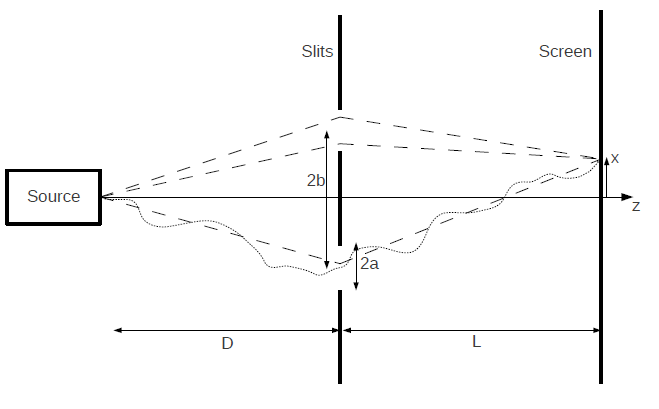
\includegraphics[width=10cm]{Imagenes/Fig8}
\caption[Esquema del experimento de la doble rendija en 2D]{Experimento de la doble rendija.}
\end{figure}
Como sabemos la probabilidad está dada por el módulo al cuadrado de la amplitud, la cual calcularemos usando el propagador. Como explicamos anteriormente hemos tomado $d=2$ en el propagador, sin embargo, vamos a explicar por qué podemos reducir aún más la complejidad del problema: consideremos la difracción por una sola rendija y que el movimiento está dividido en dos regiones, uno empezando desde la fuente y llegando a las rendijas un tiempo $T$ después de la emisión y otro de la rendija a la pantalla, este último de duración $\tau$.
\\
\\
Sin embargo, no hay nada en las leyes de la mecánica cuántica que nos diga que podemos separar el movimiento en dos tramos, esto debido a que realmente no tenemos certeza de la posición de la partícula en un tiempo $T$. En pocas palabras no sabemos cuando el electrón ha cruzado la rendija.
\\
\\
No obstante podemos considerar esta imagen clásica para estudiar el problema, veamos por qué: el electrón tiene un momentum $p_z=\hbar k_z$, el cual está relacionado con la velocidad clásica como $V_z=D/T=L/\tau$, aquí suponemos que $D$ es suficientemente grande comparado con las dimensiones en $x$ ($x,a,b\ll D,L$). Adicionalmente la longitud de onda $\lambda$ de la partícula es aproximadamente igual a la contribucion en $z$ (esto es como si tomaramos partículas que no se desvían demasiado de la trayectoria clásica). Si $\lambda \approx \lambda_z=2\pi\hbar/(mv_z)$ entonces $\lambda \ll D,L$. Esto quiere decir que el movimiento en $z$ es practicamente clásico. Note que cuánticamente es posible que el electrón pase a través de la rendija varias veces, sin embargo la probabilidad de este suceso ha de ser baja.

Teniendo en cuenta lo anterior:
\begin{eqnarray}
\nonumber K_{a,b}^{2D}((x,L+D),T+\tau;(0,0),0)&=&\int_{-\infty}^{\infty}d\omega\chi_{[b-a,b+a]}(\omega)K_{0}^{2D}((x,L+D),T+\tau;(\omega,D),T)\\
&&\nonumber \times K_{0}^{2D}((\omega,D),T;(0,0),0)\\
&=&\nonumber \frac{e^{\frac{imL^{2}}{2\hbar\tau}}}{\sqrt{2\pi i\hbar\tau/m}}\frac{e^{\frac{imD^{2}}{2\hbar T}}}{\sqrt{2\pi i\hbar T/m}}\int_{b-a}^{b+a}\frac{e^{\frac{im\omega^{2}}{2\hbar T}}}{\sqrt{2\pi i\hbar T/m}}\frac{e^{\frac{im(x-\omega)^{2}}{2\hbar\tau}}}{\sqrt{2\pi i\hbar\tau/m}}d\omega ,	
\end{eqnarray}
por tanto el propagador es el producto de dos propagadores independientes:
\begin{eqnarray}
K_z(L+D,T+\tau;0,0)&=&\frac{e^{\frac{imL^{2}}{2\hbar\tau}}}{\sqrt{2\pi i\hbar\tau/m}}\frac{e^{\frac{imD^{2}}{2\hbar T}}}{\sqrt{2\pi i\hbar T/m}}\\
K_x(x,T+\tau;0,0)&=&\int_{b-a}^{b+a}\frac{e^{\frac{im\omega^{2}}{2\hbar T}}}{\sqrt{2\pi i\hbar T/m}}\frac{e^{\frac{im(x-\omega)^{2}}{2\hbar\tau}}}{\sqrt{2\pi i\hbar\tau/m}}d\omega .
\end{eqnarray}
Una forma de comprobar que las ecuaciones (2.63) y (2.64) son correctas es ver que si quitamos las rendijas ($a\to \infty$) e integramos en $D$ en el intervalo $(-\infty,\infty)$ recuperamos el propagador de una particula libre.\\
\\
En lo que sigue nos vamos a dar a la tarea de mostrar que podemos expresar la amplitud en términos de las conocidas integrales de Fressnel, sabemos que $P(x;a,b)=|A(x;a,b)|^2$ y de (2.64):
\begin{equation}
A_1(x;a,b)=\int_{b-a}^{b+a}\frac{e^{\frac{im\omega^{2}}{2\hbar T}}}{\sqrt{2\pi i\hbar T/m}}\frac{e^{\frac{im(x-\omega)^{2}}{2\hbar\tau}}}{\sqrt{2\pi i\hbar\tau/m}}d\omega .
\end{equation} 
Organicemos de una manera diferente el exponencial de la ecuación (2.65):
\begin{eqnarray}
\nonumber \frac{m}{2\hbar\tau}(x-\omega)^{2}+\frac{m\omega^{2}}{2\hbar\tau}&=&\frac{m}{2\hbar}\left[\frac{1}{T}+\frac{1}{\tau}\right]\left[\omega^{2}-\frac{2x\omega}{\left(\frac{\tau}{T}+1\right)}+\left(\frac{x}{\frac{\tau}{T}+1}\right)^{2}-\left(\frac{x}{\frac{\tau}{T}+1}\right)^{2}\right]+\frac{mx^{2}}{2\text{\ensuremath{\hbar\tau}}}\\
&=&\nonumber \frac{m}{2\hbar}\left[\frac{1}{T}+\frac{1}{\tau}\right]\left[\omega-\frac{x}{1+\tau/T}\right]^{2}+\frac{mx^{2}}{2\text{\ensuremath{\hbar}}}\left[\frac{1}{\tau}-\frac{T}{(\tau+T)\tau}\right]\\
&=& \left[\frac{m}{2\hbar T}+\frac{m}{2\hbar\tau}\right]\left[\omega-\frac{x}{1+\tau/T}\right]^{2}+\frac{mx^{2}}{2\text{\ensuremath{\hbar}}(T+\tau)},
\end{eqnarray}
por tanto reemplazando (2.66) en (2.65)
\begin{equation}
A_{1}(x;a,b)=\frac{e^{\frac{imx^{2}}{2\hbar(T+\tau)}}}{\sqrt{2\pi i\hbar(T+\tau)/m}}\int_{b-a}^{b+a}d\omega\sqrt{\frac{T+\tau}{2\pi\hbar T\tau/m}}\ \exp\left\{ \frac{i(T+\tau)}{2\hbar T\tau/m}\left(\omega-\frac{x}{1+\tau/T}\right)^{2}\right\}
\end{equation}
Ahora si $\omega^{\prime}=\sqrt{\frac{T+\tau}{\pi\hbar T\tau/m}}\left(\omega-\frac{x}{1+\tau/T}\right)$:
\begin{equation}
\Rightarrow A_{1}(x;a,b)=\frac{e^{\frac{imx^{2}}{2\hbar(T+\tau)}}}{\sqrt{2\pi i\hbar(T+\tau)/m}}\int_{\alpha_{-}(x)}^{\alpha_{+}(x)}d\omega^{\prime}\sqrt{\frac{T+\tau}{2\pi\hbar T\tau/m}}\ \exp\left\{ \frac{i\pi\omega^{\prime 2}}{2}\right\} ,
\end{equation}
donde $\alpha_{\pm}(x)=\sqrt{\frac{T+\tau}{\pi\hbar T\tau/m}}(b\pm a)-\frac{x}{\sqrt{\pi\hbar\tau/m}}\sqrt{\frac{T}{T+\tau}}$.
Si descomponemos el exponencial de la ecuación (2.68) en su parte imaginaria y real, obtenemos las famosas integrales de Fressnel, definidas como:
\begin{equation}
C[u]\equiv \int_{0}^{u}d\omega Cos\left(\frac{\pi\omega ^2 }{2}\right)\hspace{0.3cm} ;\hspace{0.3cm} S[u]\equiv \int_{0}^{u}d\omega Sin\left(\frac{\pi\omega ^2 }{2}\right) .
\end{equation}
Así:
\begin{eqnarray}
&\nonumber A_{1}(x;a,b)=\frac{e^{\frac{imx^{2}}{2\hbar(T+\tau)}}}{\sqrt{(2i)^{2}\pi\hbar(T+\tau)/m}}\\
&\times[C[\alpha_{+}(x;a.b)]-C[\alpha_{-}(x;a.b)]+iS[\alpha_{+}(x;a.b)]-iS[\alpha_{-}(x;a.b)]]\\
&A_{2}(x;a,b)=A_{1}(x;a,-b).
\end{eqnarray}
Para dos rendijas podemos calcular la amplitud total simplemente sumando:
\begin{equation}
A(x;a,b)=A_{1}(x;a,b)+A_{2}(x;a,b).
\end{equation}


\subsection{Difracción por una rendija.}
En el caso de una sola rendija tenemos que $b=0$, además recordando que $\lambda\approx\lambda_z=h/mv_z$ ; $v_z=L/\tau=D/T$, podemos escribir:
\begin{equation}
\alpha(x,a)=\sqrt{N_F(a)}\sqrt{1+L/D}\left[	1-\frac{x}{a(1+L/D)}\right] \hspace{0.3cm};\hspace{0.3cm} N_F(a)=2a^2/\lambda L .
\end{equation}
Las integrales de Fressnel tienen un comportamiento diferente dependiendo del valor de $N_F(a)$:
\begin{eqnarray}
C(\pm u)&=&\pm\frac{1}{2}+\frac{1}{\pi u}Sin\left(\frac{\pi u^2}{2}\right),\hspace{0.3cm}u\geq 1\\
S(\pm u)&=&\pm\frac{1}{2}-\frac{1}{\pi u}Sin\left(\frac{\pi u^2}{2}\right),\hspace{0.3cm}u\geq 1 .
\end{eqnarray}
Definiendo $\eta\equiv 1+L/D$ y $\gamma=\eta-1$, en el caso $\frac{x}{a\eta}-1\gg\frac{1}{\sqrt{N_F(a)\eta}}$ encontramos que:
\begin{eqnarray}
\alpha(x,a)&\ll&-1\\
\alpha(x,-a)&\gg&1 ,
\end{eqnarray} 
por tanto:
\begin{eqnarray}
C[\alpha(x,\pm a)]&=&\pm\frac{1}{2}+\frac{1}{\pi\alpha(x,\pm a) }Sin\left(\frac{\pi \alpha(x,\pm a)^2}{2}\right)\\
S[\alpha(x,\pm a)]&=&\pm\frac{1}{2}-\frac{1}{\pi\alpha(x,\pm a) }Sin\left(\frac{\pi \alpha(x,\pm a)^2}{2}\right) .
\end{eqnarray}
Es fácil mostar que $C[\alpha_-(x,a,o)]=-C[\alpha(x,-a)]$ y $S[\alpha_-(x,a,o)]=-S[\alpha(x,-a)]$, con esto, y usando la ecuación (2.70):
\begin{eqnarray}
\nonumber & P^{\text{(1rendija)}}(x;a,b)=|A(x;a,b)|^2=\\&\frac{1}{2\lambda(L+D)}
([C(\alpha(x,a))+C(\alpha(x.-a))]^{2}+[S(\alpha(x.a))+S(\alpha(x.-a))]^{2}) .
\end{eqnarray}
Usando las ecuaciones (2.78),(2.79) y (2.80) encontramos:
\begin{equation}
P^{(\text{1rendija})}(x,a)\simeq\frac{2\gamma}{\pi^{2}\eta^{2}}\left(\frac{a^{2}}{\left(\frac{x^{2}}{\eta^{2}}-a^{2}\right)^{2}}+\frac{1}{\left(\frac{x^{2}}{\eta^{2}}-a^{2}\right)}\text{Sin}^{2}\left(\pi N_{F}(a)\frac{x}{a}\right)\right) ,
\end{equation}
en el límite $N_F(a)\ll 1\Rightarrow \frac{x}{\eta}\gg a$ ,tenemos la siguiente aproximación:
\begin{equation}
P^{(\text{1rendija})}(x,a)\simeq\frac{2\gamma}{\pi^{2}x^{2}}\text{Sin}^{2}\left(\pi N_{F}(a)\frac{x}{a}\right) .
\end{equation}
Este límite es conocido como el régimen de Fraunhofer (Pantalla lejana), Figura 2.9. Es importante recalcar que en el regimen intermedio $(N_F(a)\approx 1)$, las aproximaciones (2.81) y (2.82) siguen siendo válidas.
\begin{figure}[h]
\centering
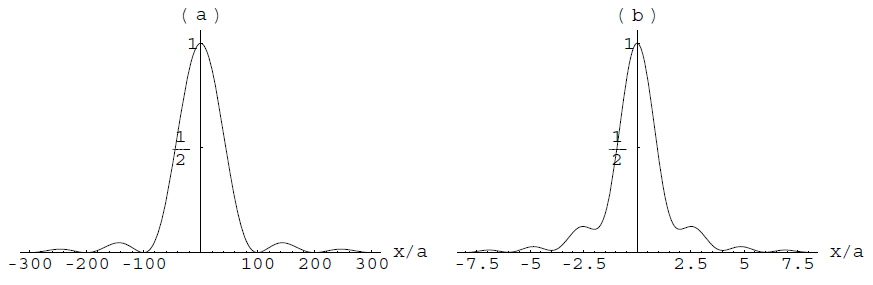
\includegraphics[width=13cm]{Imagenes/Fig9}
\caption[Patron de interferencia, 1 rendija, regimen de Fraunhofer]{Curva de difracción para una sola rendija, en la figura (a) $N_F(a)=0.01$, en (b) $N_F(a)=0.5$. Tomado de [1]}
\end{figure}
Sin embargo para $N_F(a)\ll 1$, obtenemos diferentes aproximaciones asintóticas:
\begin{eqnarray}
\nonumber &P^{(\text{1rendija})}(x)\simeq\frac{\gamma}{\eta}\left(\frac{\sqrt{N_{F}(a)}}{2a}+\frac{\text{\text{Sin}}\left(\frac{\pi}{2}N_{F}(a)\eta\left(1-\frac{x}{a\eta}\right)^{2}\right)}{2\pi\sqrt{\eta}\left(a-\frac{x}{\eta}\right)}+\frac{\text{\text{Sin}}\left(\frac{\pi}{2}N_{F}(a)\eta\left(1+\frac{x}{a\eta}\right)^{2}\right)}{2\pi\sqrt{\eta}\left(a+\frac{x}{\eta}\right)}\right)^{2}\\
&+\frac{\gamma}{\eta}\left(\frac{\sqrt{N_{F}(a)}}{2a}-\frac{\text{\text{Cos}}\left(\frac{\pi}{2}N_{F}(a)\eta\left(1-\frac{x}{a\eta}\right)^{2}\right)}{2\pi\sqrt{\eta}\left(a-\frac{x}{\eta}\right)}-\frac{\text{\text{Cos}}\left(\frac{\pi}{2}N_{F}(a)\eta\left(1+\frac{x}{a\eta}\right)^{2}\right)}{2\pi\sqrt{\eta}\left(a+\frac{x}{\eta}\right)}\right)^{2},|x|<a\eta ,
\end{eqnarray}
\begin{equation}
P^{(\text{1rendija})}(x,a)\simeq\frac{2\gamma}{\pi^{2}\eta^{2}}\left(\frac{a^{2}}{\left(\frac{x^{2}}{\eta^{2}}-a^{2}\right)^{2}}+\frac{1}{\left(\frac{x^{2}}{\eta^{2}}-a^{2}\right)}\text{Sin}^{2}\left(\pi N_{F}(a)\frac{x}{a}\right)\right), |x|>a\eta .
\end{equation}
Esto se debe a que las aproximaciones asintóticas tienen el siguiente comportamiento:
\begin{eqnarray}
&\alpha(x,\pm a)\gg 1,\hspace{0.2cm} \text{si}\hspace{0.2cm} N_F(a)\gg 1 \hspace{0.2cm} \text{y}\hspace{0.2cm} |x|<a\eta\\
&\pm\alpha(x,\mp a)\gg 1,\hspace{0.2cm} \text{si}\hspace{0.2cm} N_F(a)\gg 1 \hspace{0.2cm} \text{y}\hspace{0.2cm} |x|>a\eta .
\end{eqnarray}
La función (2.83) oscila rápidamente alrededor del valor constante $N_F(a)\gamma/2a^2\eta=1/(\lambda_z(L+D))$ en $|x|<a\eta$ y la función (2.84) decrece rapidamente a 0 en $|x|>a\eta$. La curva de difracción se muestra en la figura 2.10.
\begin{figure}[h!]
\centering
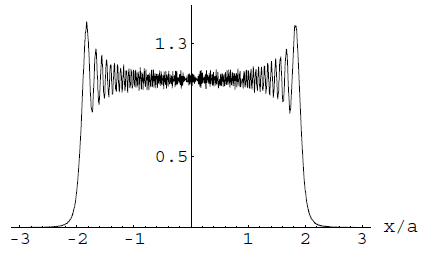
\includegraphics[width=10cm]{Imagenes/Fig10}
\caption[Patrón de interferencia, 1 rendija, regimen de Fressnel]{Curva de difracción para una sola rendija, en la figura  $N_F(a)=100$. Tomado de [1]}
\end{figure}



\subsection{Interferencia y difracción por dos rendijas.}

Podemos calcular la curva de difracción e interferencia para dos rendijas usando la siguiente expresión:
\begin{equation}
P^{(2\text{rendija})}(x;a,b)=P_{1}(x;a,b)+P_{2}(x;a,b)+I_{12}(x;a,b) ,
\end{equation}
donde:
\begin{eqnarray}
\nonumber P_{1}(x;a,b)&=&|A_1(x;a,b)|^2\\
\nonumber &=&\frac{\gamma}{2\lambda L\eta}([C(\alpha_{+}(x;a,b)-C(\alpha(x;a,b))]^{2}+[S(\alpha_{+}(x;a,b)-S(\alpha(x;a,b))]^{2})\\
P_2(x;a,b)&=&|A_2(x;a,b)|^2=P_1(x;a,-b) ,
\end{eqnarray}
y el término de interferencia:
\begin{eqnarray}
\nonumber I_{12}(x;a,b)&=& A_1(x;a,b)A_2(x;a,b)^*+A_2(x;a,b)A_1(x;a,b)^*\\
\nonumber &=&\frac{\gamma}{\lambda L\eta}([C(\alpha_{+}(x;a,b)-C(\alpha(x;a,b))][C(\alpha_{+}(x;a,-b)-C(\alpha(x;a,-b))]\\
&+& [S(\alpha_{+}(x;a,b)-S(\alpha(x;a,b))][S(\alpha_{+}(x;a,-b)-S(\alpha(x;a,-b))]) .
\end{eqnarray}
Hay que notar que en el caso de dos rendijas hay un término adicional, llamado el \textit{término de interferencia}, este es similar al encontrado en óptica. Esto resulta en un efecto de modulación de la curva de difracción dada por la suma de los términos de la ecuación (2.88).\\
\\
Definamos los números de Fressnel:
\begin{equation}
N_F(a)\equiv 2a^2/\lambda_zL ;\hspace{0.3cm} N_F(b)\equiv 2b^2/\lambda_zL ;\hspace{0.3cm} N_F\equiv 2ab/\lambda_zL=\sqrt{N_F(a)N_F(b)/2} ,
\end{equation}
en el caso de dos rendijas de ancho $2a$ y separadas por una distancia $2b$, en el caso en que $b\gg a$ tenemos los siguientes comportamientos, que se dividen en dos fases:
\begin{itemize}
\item Si $N_F\ll 1$, estamos en la \textit{fase mezclada}, es decir, encontramos una curva de interferencia modulada por la curva de difración de una rendija de tamaño $a$. En este caso estamos en el regimen de Fressnel, $N_F(a)\ll 1$. Este se muestra en la figura 2.11(a). 
\item Si $N_F\gg 1$, estamos en la \textit{fase separada}, es decir, hay dos curvas de interferencia, moduladas por las curvas de difracción correspondientes a cada rendija, cada curva centrada en $\pm b\eta$.	La forma de las curvas de difracción dependen de $N_F(a)$ y son similares al caso de una rendija (donde teniamos dos regímenes establecidos: Fressnel y Fraunhofer). En la figura 2.11(c), $N_F(a)\ll 1$ y en la figura 2.11(d) $N_F(a)\gg 1$.
\item Si $N_F\sim 1$ observamos una separación entre dos curvas de interferencia, moduladas por una curva de difracción que corresponde al de una rendija en el caso de regimen intermedio, esto se muestra en la figura 2.11(b). 
\end{itemize}
\begin{figure}[h!]
\centering
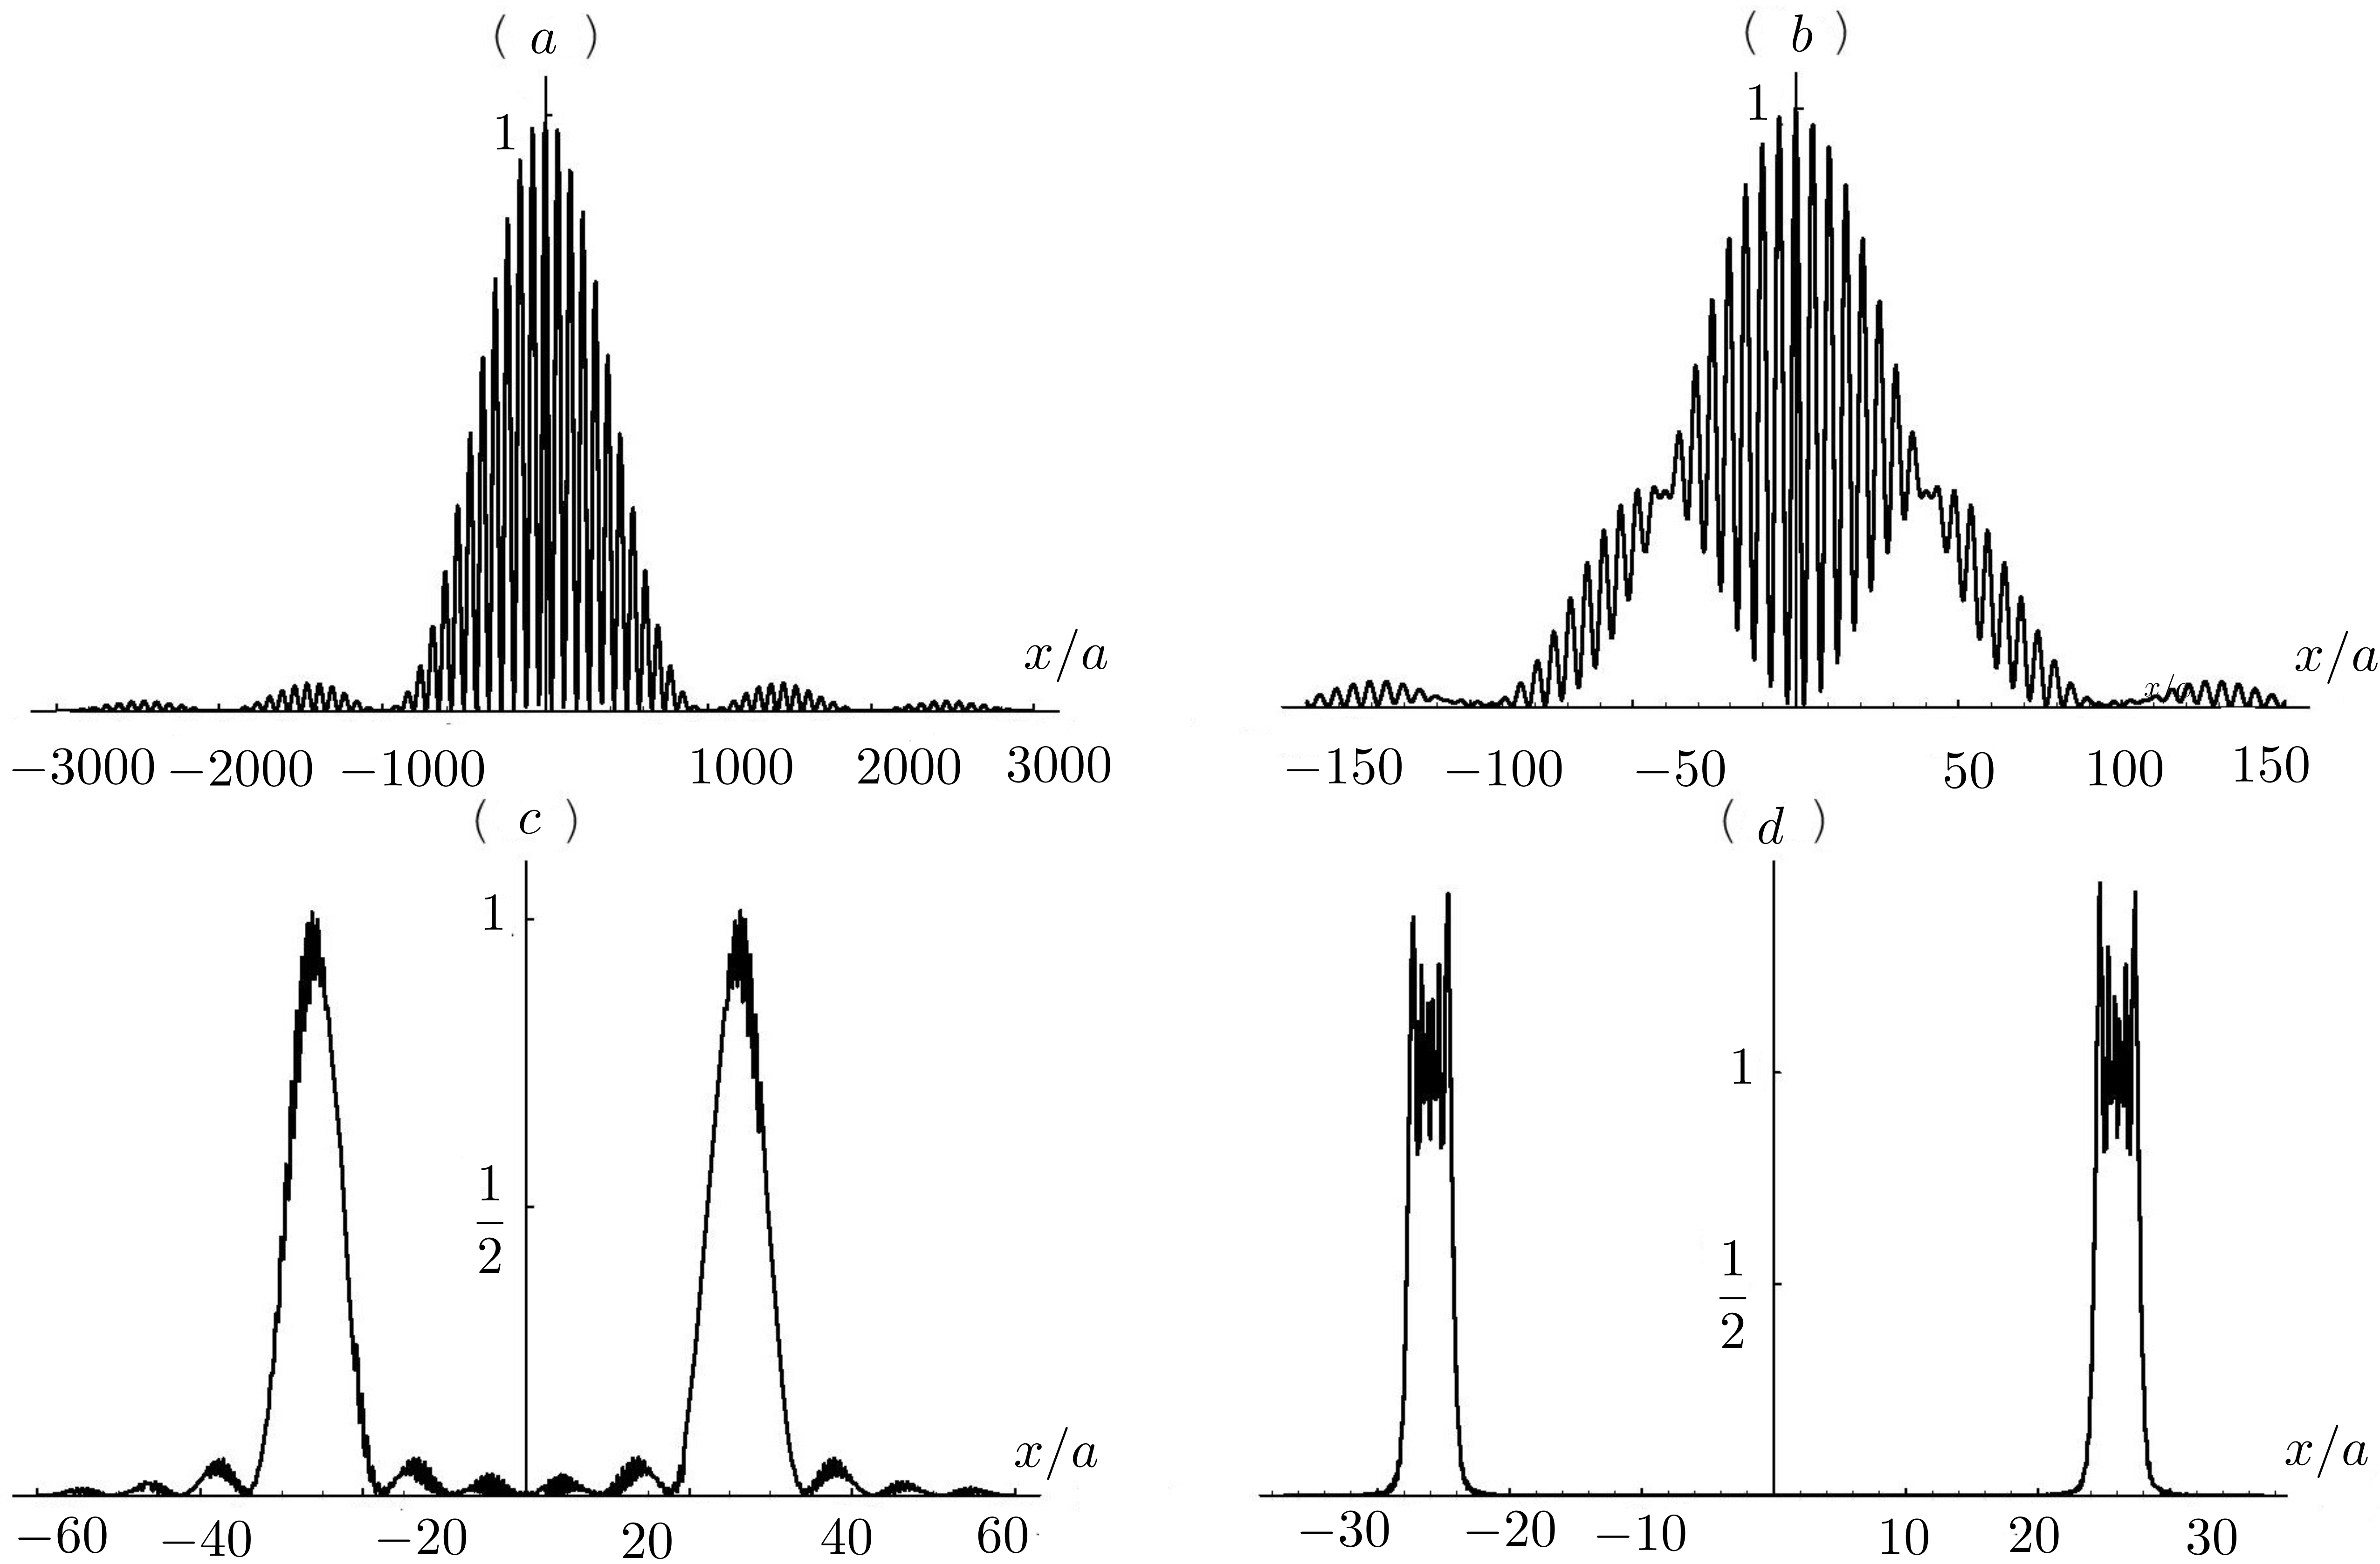
\includegraphics[width=14.5cm]{Imagenes/Fig11}
\caption[Patrón de interferencia, 2 rendijas]{Curva de difracción para dos rendijas, en la figura  $N_F(a)=0.001$ para (a), 0.015 para (b), 0.12 para (c), 6 para (d) . Tomado de [1]}
\end{figure}
\newpage
\newpage





\section{Campos escalares.}
En analogía con lo estudiado en la sección anterior para una partícula, definimos la transición vacío-vacío en presencia de una fuente $J(x)$ para un campo $\phi(x)$ como:
\begin{equation}
Z[J]=\int\mathcal{D}\phi\ \exp\left\{ i\int d^{4}x\left[\mathcal{L}(\phi)+J(x)\phi(x)+\frac{i}{2}\epsilon\phi^{2}(x)\right]\right\} .
\end{equation}
En este caso en vez de dividir el espacio-tiempo en segmentos, dividimos el espacio 4 dimensional (4D) de Minkowski en hipervolúmenes (4D) asumiendo que en cada uno de estos volúmenes $\phi(x)$ es constante. Si $\mathcal{L}=\mathcal{L}(Klein-Gordon)=\frac{1}{2}(\partial_\mu\phi\partial^\mu\phi-m^2 \phi^2)$, tenemos:
\begin{equation}
Z_{0}[J]=\text{\ensuremath{\int\mathcal{D}}}\phi\ \exp\left\{ i\int d^{4}x\left[\frac{1}{2}(\partial_{\mu}\phi\partial^{\mu}\phi-(m^{2}-i\epsilon)\phi^{2}))+J\phi\right]\right\} .
\end{equation} 	
Ahora como $\int\partial_{\mu}\phi\partial^{\mu}\phi=\int\partial_{\mu}(\phi\partial^{\mu}\phi)-\int\phi\square\phi=0-\int\phi\square\phi$, donde hemos usado que la primera integral es una cuadridivergencia y puede ser expresada como una integral de superficie, y poniendo la condición de frontera de que los campos se anulan en el borde, este término es cero. Por tanto (2.92) queda:
\begin{equation}
Z_{0}[J]=\text{\ensuremath{\int\mathcal{D}}}\phi\ \exp\left\{ -i\int d^{4}x\left[\frac{1}{2}(\phi\square\phi+(m^{2}-i\epsilon)\phi^{2}))-J\phi\right]\right\} .
\end{equation}
El campo $\phi(x)$ no satisface la ecuacion de K-G. Para evaluar $Z_0[J]$ separemos $\phi(x)$:
\begin{equation}
\phi \rightarrow \phi(x)+\phi_0(x) ,
\end{equation}
se puede probar fácilmente que $\int\phi_{0}(\square+m^{2}-i\epsilon)\phi=\int\phi(\square+m^{2}-i\epsilon)\phi_{0}$, por tanto:
\begin{eqnarray}
\nonumber \int d^{4}x\left[\frac{1}{2}\phi(\square+m^{2}-i\epsilon)\phi-J\phi\right]&\rightarrow\int d^{4}x[\frac{1}{2}\phi(\square+m^{2}-i\epsilon)\phi+\phi(\square+m^{2}-i\epsilon)\phi_{0}\\
&+\frac{1}{2}\phi_{0}(\square+m^{2}-i\epsilon)\phi_{0}-J\phi-J\phi_{0}],
\end{eqnarray}
si ahora escogemos $\phi_0$ tal que satisfaga:
\begin{equation}
(\square+m^2-i\epsilon)\phi_0(x)=J(x),
\end{equation}
entonces (2.95) queda como:
\begin{equation}
\int d^{4}x\left[\frac{1}{2}\phi(\square+m^{2}-i\epsilon)\phi-\frac{1}{2}J\phi_{0}\right].
\end{equation}
La solución a (2.96) es:
\begin{equation}
\phi_{0}(x)=-\int\triangle_{F}(x-y)J(y)d^{4}y ,
\end{equation}
donde $\triangle_F(x-y)$, llamado el propagador de Feynmann, es la función de green del operador $(\square+m^2-i\epsilon)$ y cumple:
\begin{equation}
(\square+m^2-i\epsilon)\triangle_{F}(x)=-\delta^4(x).
\end{equation}
Con todo lo anterior podemos escribir $Z_0[J]$ como:
\begin{equation}
Z_0[J]=\ \exp\left\{ -\frac{i}{2}\int d^{4}xd^{4}yJ(x)\triangle_{F}(x-y)J(y)\right\} \int\mathcal{D}\phi\ \exp\left\{ -\frac{i}{2}\int d^{4}x\left[\frac{1}{2}(\phi(\square +m^{2}-i\epsilon)\phi\right]\right\} .
\end{equation}
Por tanto hemos logrado separar el funcional generatriz en dos partes, una que depende unicamente de $J(x)$ y otra de $\phi(x)$, esta última de hecho es simplemente un número que llamaremos $\mathcal{N}$, así:
\begin{equation}
Z_{0}[J]=\mathcal{N}\ \exp\left\{ -\frac{i}{2}\int d^{4}xd^{4}yJ(x)\triangle_{F}(x-y)J(y)\right\} .
\end{equation}
\subsection{Integración funcional.}
Vamos a generalizar la fórmula de integración Gaussiana a $n$ variables discretas para luego analizar este tipo de fórmulas en el caso de cálculo funcional. Sabemos que 
\begin{equation}
\int_{-\infty}^{\infty}e^{-\frac{1}{2}ax^{2}}dx=\left(\frac{2\pi}{a}\right)^{1/2}\Rightarrow\int\ \exp\left(-\frac{1}{2}\sum a_{n}x_{n}^{2}\right)dx_{1}...dx_{n}=\frac{(2\pi)^{n/2}}{\prod_{i=1}^{n}a_{i}^{1/2}} .
\end{equation}
Sea $A$ una matriz diagonal y $x$ un vector, el producto escalar de $Ax$ y $x$ es $(x,Ax)=\sum_n a_nx_{n}^{2}$ y $det(A)=\prod_{i=1}^{n}a_i$. Por tanto podemos escribir (2.102) como:
\begin{equation}
\int\ \exp\left[-\frac{1}{2}(x,Ax)\right]d^{n}x=(2\pi)^{n/2}(detA)^{-1/2} .
\end{equation}
Si definimos la medida $dx=d^nx(2\pi)^{-n/2}$, tenemos:
\begin{equation}
\int\ \exp\left[-\frac{1}{2}(x,Ax)\right]dx=(detA)^{-1/2} ,
\end{equation}
esta ecuación puede ser extendida a formas cuadráticas $Q(x)=\frac{1}{2}(x,Ax)+(b,x)+c$. En este caso tenemos:
\begin{equation}
\int\ \exp\left[-\frac{1}{2}\left\{ (x,Ax)+(b,x)+c\right\} \right]dx=\ \exp\left[\frac{1}{2}(b,A^{-1}b)-c\right]det(A)^{-1/2} .
\end{equation}
La generalización funcional de la ecuación (2.104) es:
\begin{equation}
\int\mathcal{D}\phi\ \exp\left[-\frac{1}{2}\int\phi(x)A\phi(x)dx\right]=(detA)^{-1/2} .
\end{equation}
Así si partimos de $Z_{0}[J]=\int\mathcal{D}\phi\ \exp\left\{ -i\int\left[\frac{1}{2}\phi(\square+m^{2}-i\epsilon)\phi-J\phi\right]d^{4}x\right\} $ y aplicando (2.105) y (2.106) con $A=i(\square+m^2-i\epsilon)$, $b=-iJ(x)$ y $c=0$. Tenemos:
\begin{equation}
Z_{0}[J]=\ \exp\left[\frac{i}{2}\int J(x)(\square+m^{2}-i\epsilon)^{-1}J(y)dxdy\right]det(i(\square+m^{2}-i\epsilon))^{-1/2} .
\end{equation}
Como sabemos  de (2.99) $(\square +m^2-i\epsilon)^{-1}=-\triangle_F(x-y)$ y con la ecuación (2.106):
\begin{equation}
Z_0[J]=\ \exp\left\{ -\frac{i}{2}\int d^{4}xd^{4}yJ(x)\triangle_{F}(x-y)J(y)\right\} \int\mathcal{D}\phi\ \exp\left\{ -\frac{i}{2}\int d^{4}x\left[\frac{1}{2}(\phi(\square +m^{2}-i\epsilon)\phi\right]\right\} . 
\end{equation}
Esta es la misma ecuación que (2.100)!

\subsection{Funciones de Green de la partícula libre.}
Si expandimos la amplitud de transición en serie:
\begin{equation}
Z_{0}[J]=\mathcal{N}\left\{ 1-\frac{i}{2}\int dxdyJ(x)\triangle_{F}(x-y)J(y)+\frac{1}{2!}\left(\frac{i}{2}\right)^{2}\left[\int d^{4}xd^{4}yJ(x)\triangle_{F}(x-y)J(y)\right]^{2}+...\right\},
\end{equation}
e introduciendo la transformada de Fourier de $J(x)$, 
\begin{equation}
J(x)=\int J(p)e^{-ip\cdot x}d^4p,
\end{equation}
teniendo en cuenta que para abreviar hemos escrito los diferenciales en el cuadrivolumen como $d^4h\equiv dh$, tenemos:
\begin{eqnarray}
\nonumber -\frac{i}{2}\int J(x)\triangle_F(x-y)J(y)dxdy&=&-\frac{i}{2(2\pi)^{4}}\int\frac{J(p_{1})e^{-ip_{1}\cdot x}J(p_{2})e^{-ip_{2}\cdot y}e^{-ik(x-y)}dxdydkdp_{1}dp_{2}}{k^{2}-m^{2}+i\epsilon}\\
\nonumber &=& -\frac{i}{2(2\pi)^{4}}\int\frac{J(p_{1})J(p_{2})e^{-ix(p_{1+k})}e^{-iy(p_{2}-k)}dxdydkdp_{1}dp_{2}}{k^{2}-m^{2}+i\epsilon}.\\
\nonumber \text{Integrando en x,y} &&\\
\nonumber &=& -\frac{i(2\pi)^{8}}{2(2\pi)^{4}}\int\frac{J(p_{1})J(p_{2})\delta(p_{1}+k)\delta(p_{2}-k)dkdp_{1}dp_{2}}{k^{2}-m^{2}+i\epsilon}\\
&=& -\frac{i(2\pi)^{4}}{2}\int\frac{J(k)J(-k)d^{4}k}{k^{2}-m^{2}+i\epsilon}.
\end{eqnarray}
Si identificamos la expresión anterior mediante las reglas de la figura 2.12,
\begin{SCfigure}[1][h]
\caption[Diagrama de Feynmann segunda cuantización]{Diagrama de Feynmann segunda cuantización}
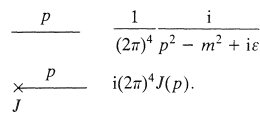
\includegraphics[width=5.5cm]{Imagenes/Fig12}
\end{SCfigure}
entonces la integral (2.111) puede ser identificada con el diagrama que aparece en la figura 2.13:
\begin{SCfigure}[1][h!]
\caption[Diagrama de Feynmann segunda cuantización]{Representación de (2.111)}
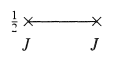
\includegraphics[width=3cm]{Imagenes/Fig13}
\end{SCfigure}
\\
\\
\\
por tanto finalmente:
\begin{equation}
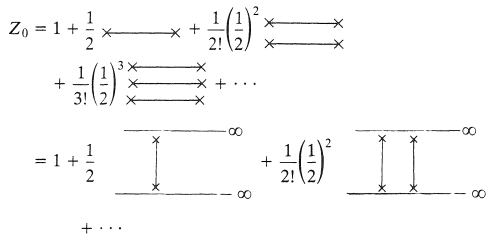
\includegraphics[width=12cm]{Imagenes/Fig14}
\end{equation}
Podemos interpretar esta serie como la propagación y posterior aniquilación de  una partícula entre fuentes, de dos partículas entre fuentes y así sucesivamente. Tenemos por tanto una teoría de muchos cuerpos, lo cual es consistente con nuestra idea inicial de utilizar un campo. Cada término en la serie es una función de Green por tanto $Z_0[J]$ es llamada un \textit{funcional generatriz} para las funciones de Green de la teoría.
\\
\\
Para entender esto analicemos la expansión en series de un funcional, primero recordemos la expansion en series de una funcion de $k$ variables $F(y_1,...,y_k)$:
\begin{equation}
F\{y\}=F(y_{1},..,y_{k})=\sum_{n=0}^{\infty}\sum_{i_{1}}^{k}...\sum_{i_{n}}^{k}\frac{1}{n!}T_{n}(i_{1},...,i_{n})y_{i_{1}}...y_{i_{n}},
\end{equation}
donde
\begin{equation}
T_{n}(i_{1},...,i_{n})=\frac{\partial F\{y\}}{\partial y_{1}...\partial y_{n}}|_{y=0} .
\end{equation}
Si vamos al caso de muchas variables continuas $i\rightarrow x_1, y_i\rightarrow y(x),\sum_i\rightarrow \int dx$, entonces obtenemos la serie de potencias de un funcional:
\begin{equation}
F[y]=\sum_{n=0}^{\infty}\int dx_{1}...dx_{n}\frac{1}{n!}T_{n}(x_{1},...,x_{n})y(x_{1})...y(x_{n}),
\end{equation}
y en este caso:
\begin{equation}
T_{n}(x_{1},...,x_{n})=\frac{\delta}{\delta y(x_{1})}...\frac{\delta}{\delta y(x_{n})}F[y]|_{y=0} .
\end{equation}
$F[y]$ es llamado el \textit{funcional generatriz} de las funciones  $T_{n}(x_{1},...,x_{n})$. Si escogemos una normalización tal que $Z_0[J]|_{J=0}=1 \Rightarrow \mathcal{N}=1$, por tanto:
\begin{equation}
Z_{0}[J]=\ \exp\left\{ -\frac{i}{2}\int dxdyJ(x)\triangle_{F}(x-y)J(y)\right\} .
\end{equation}
Asi $Z_0[J]$ es el funcional generatriz de:
\begin{equation}
\tau(x_{1},...,x_{n})=\frac{1}{i^{n}}\frac{\delta^{n}Z_{o}[J]}{\delta J(x_{1})...\delta J(x_{n})}|_{J=0}.
\end{equation}
En analogía con la ecuación (2.56) tenemos:
\begin{equation}
\frac{\delta^{n}Z_{o}[J]}{\delta J(x_{1})...\delta J(x_{n})}|_{J=0}=i^{n}\langle0|T[\phi(x_{1})...\phi(x_{n})]|0\rangle ,
\end{equation}
entonces:
\begin{equation}
\tau(x_1,...,x_n)=\langle0|T[\phi(x_{1})...\phi(x_{n})]|0\rangle .
\end{equation}
A las funciones $\tau(x_1,...,x_n)$ se les llama funciones de Green o funciones de n-puntos, calculemos algunas, empecemos con la función de 2-puntos:
\begin{equation}
\tau(x,y)=-\frac{\delta^2Z_0[J]}{\delta J(x)\delta J(y)}|_{J=0} ,
\end{equation}
\begin{eqnarray}
\nonumber \Rightarrow \frac{1}{i}\frac{\delta Z_{0}[J]}{\delta J(x)}&=&-\int\triangle_{F}(x-x_{1})J(x_{1})\times\ \exp\left\{ -\frac{i}{2}\int dxdy\text{\ensuremath{\triangle}}_{F}(x_{1}-x_{2})J(x_{1})J(x_{2})\right\}\\
\nonumber &=& -\int\triangle_{F}(x-x_{1})J(x_{1})\text{\ensuremath{\times}Exp}\left\{ \frac{-i}{2}\int J\triangle_{F}J\right\} ,\\ 
\nonumber \Rightarrow \frac{1}{i}\frac{\delta}{\delta J(y)}\frac{1}{i}\frac{\delta Z_{0}[J]}{\delta J(x)}&=&\int\triangle_{F}(x-x_{1})J(x_{1})\int\triangle_{F}(y-x_{1})J(x_{1})\text{\ensuremath{\times}Exp}\left\{ \frac{-i}{2}\int J\triangle_{F}J\right\}\\
&&+ i\triangle_{F}(x-y)\text{\ensuremath{\times}Exp}\left\{ \frac{-i}{2}\int J\triangle_{F}J\right\} ,
\end{eqnarray}
evaluando en $J=0$ la expresión (2.122) tenemos:
\begin{equation}
\tau(x,y)=i\triangle_F(x-y) .
\end{equation}
Pero, ¿cuál es el significado físico de esta expresión? Sabemos que:
\begin{equation}
\tau(x,y)=\langle0|T[\phi(x)\phi(y)]|0\rangle=\Theta(x_{0}-y_{0})\langle0|\phi(x)\phi(y)|0\rangle+\Theta(y_{0}-x_{0})\langle0|\phi(y)\phi(x)|0\rangle ,
\end{equation}          
si descomponemos el campo $\phi(x)$ como:
\begin{eqnarray}
\phi^{(+)}(x)&=&\int\frac{d^{3}k}{[(2\pi)^{3}2\omega_{k}]^{1/2}}f_{k}(x)a(k)\\
\phi^{(-)}(x)&=&\int\frac{d^{3}k}{[(2\pi)^{3}2\omega_{k}]^{1/2}}f_{k}^*(x)a^\dagger(k),
\end{eqnarray}
y reemplazamos en (2.125), la expresión que sobrevive es:
\begin{equation}
\tau(x,y)=\Theta(x_{0}-y_{0})\langle0|\phi^{(+)}(x)\phi^{(-)}(y)|0\rangle+\Theta(y_{0}-x_{0})\langle0|\phi^{(+)}(y)\phi^{(-)}(x)|0\rangle .
\end{equation}
Estas son las amplitudes para un partícula que es creada en el evento $(y_0,y)$, se propaga y es posteriormente destruida en $(x_0,x)$ o una partícula que es creada en el evento $(x_0,x)$, se propaga y es posteriormente destruida en $(y_o,y)$. Lo anterior se ve representado en la figura 2.14.
\begin{figure}[h!]
\centering
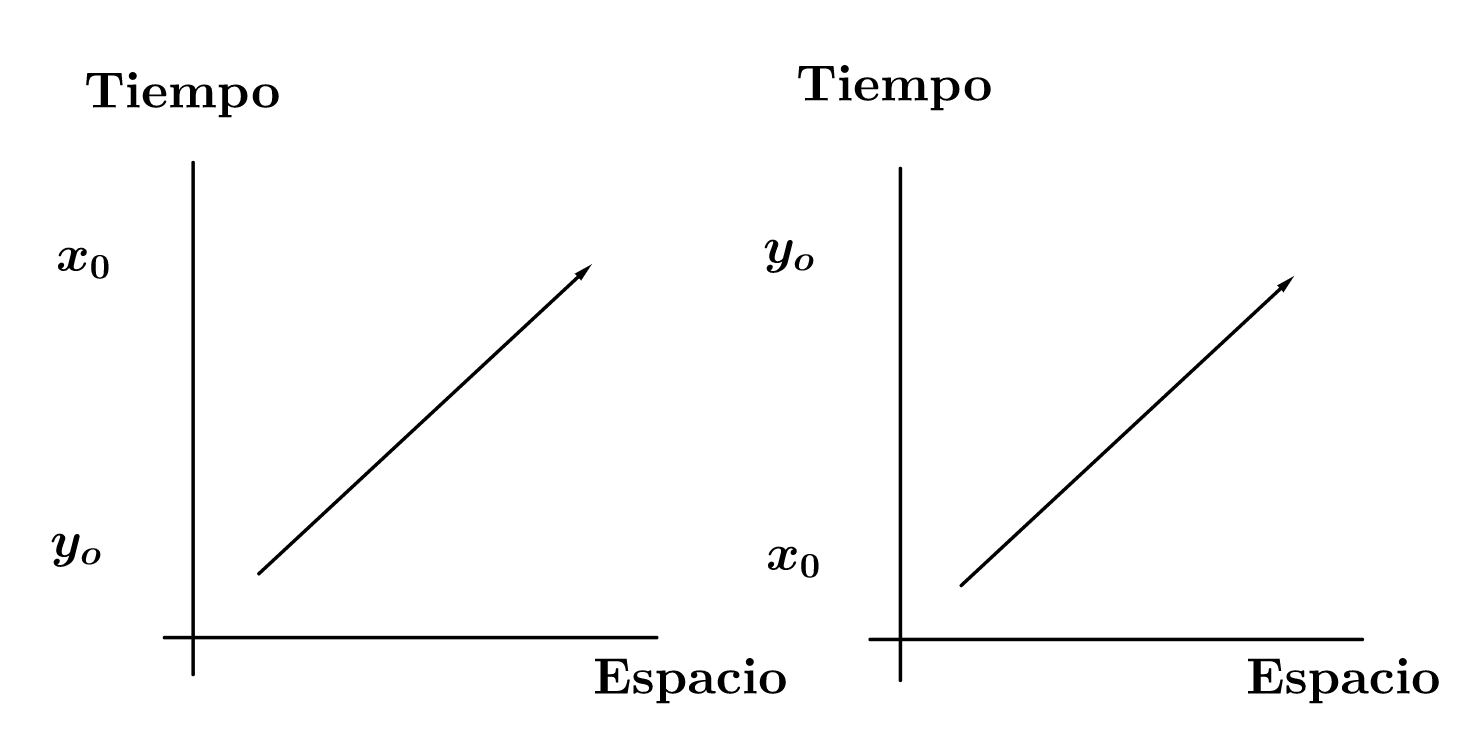
\includegraphics[width=11cm]{Imagenes/Fig15}
\caption[Representación gráfica de la función de 2-puntos ]{Representación gráfica de la ecuación 2.127}
\end{figure}
\\
\\
Es claro ahora que la función de 1-punto es:
\begin{equation}
\tau(x)=\langle 0|\phi(x)|0\rangle=0 .
\end{equation}
Calculemos entonces la función de 3-puntos, partiendo de (2.122):
\begin{eqnarray}
\nonumber\left(\frac{1}{i}\right)^{3}\frac{\delta}{\delta J_{1}}\frac{\delta}{\delta J_{2}}\frac{\delta}{\delta J_{3}}Z_{0}[J]&=&-i\triangle_{F}(x_{3}-x_{2})\int\triangle_{F}(x_{1}-x)J(x)dx\ \exp\left\{ \frac{-i}{2}\int J\triangle_{F}J\right\}\\
\nonumber && -i\triangle_{F}(x_{2}-x_{1})\int\triangle_{F}(x_{3}-x)J(x)dx\ \exp\left\{ \frac{-i}{2}\int J\triangle_{F}J\right\}\\
\nonumber &&-i\triangle_{F}(x_{3}-x_{1})\int\triangle_{F}(x_{2}-x)J(x)dx\ \exp\left\{ \frac{-i}{2}\int J\triangle_{F}J\right\}\\
\nonumber &&-\int\triangle_{F}(x_{3}-x)J(x)dx\int\triangle_{F}(x_{2}-x)J(x)dx\\
&&\times\int\triangle_{F}(x_{1}-x)J(x)dx\ \exp\left\{ \frac{-i}{2}\int J\triangle_{F}J\right\} ,
\end{eqnarray}
si evaluamos en $J=0$ la ecuación (2.129) vemos que $\tau(x_1,x_2,x_3)=0$. Para encontrar la función de 4-puntos derivamos de nuevo, los términos que sobreviven al hacer $J=0$ son:
\begin{eqnarray}
\nonumber \tau(x_1,x_2,x_3,x_4)&=&\langle 0|T[\phi(x_1)\phi(x_2)\phi(x_3)\phi(x_4)]|0\rangle\\
\nonumber &&-[\triangle_{F}(x_{3}-x_{2})\triangle_{F}(x_{1}-x_{4})\\
\nonumber &&+\triangle_{F}(x_{2}-x_{1})\triangle_{F}(x_{3}-x_{4})\\
&&+\triangle_{F}(x_{3}-x_{1})\triangle_{F}(x_{2}-x_{4})].
\end{eqnarray}
La ecuación (2.130) es el producto de funciones de 2-puntos:
\begin{equation}
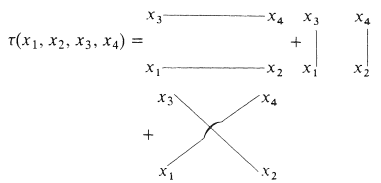
\includegraphics[width=8cm]{Imagenes/Fig16}.
\end{equation}
Así uno puede darse cuenta que si $n$ es impar la función de n-puntos se anula y si es par, es la suma de los productos de las diferentes permutaciones de funciones de 2-puntos.


\subsection{Funcional generatriz para campos interactuantes.}
Ahora debemos lidiar con el problema de encontrar el funcional generatriz para el caso de una teoría con términos de interacción en $\mathcal{L}$, en general para campos escalares $\mathcal{L}=\frac{1}{2}\left[\partial_{\mu}\phi\partial^{\mu}\phi-m^{2}\phi^{2}\right]+\mathcal{L}_{int}$. El funcional generatriz normalizado, con $S=\int \mathcal{L}dx$ es:
\begin{equation}
\frac{\int\mathcal{D}\phi\ \exp\left(iS+\int J\phi dx\right)}{\int\mathcal{D}\phi\ \exp\left(iS\right)} .
\end{equation}
Por tanto queremos encontrar la ecuación diferencial que obedece $Z[J]$ y resolverla en términos de $Z_0[J]$. Para esto primero veamos la ecuación diferencial que satiscace $Z_0[J]$. Sabemos que:
\begin{equation}
\frac{1}{i}\frac{\delta Z_{0}[J]}{\delta J(x)}=-\int\triangle_{F}(x-y)J(y)dy\ \exp\left\{ \frac{-i}{2}\int J\triangle_{F}Jdxdy\right\} ,
\end{equation}
por tanto, si aplicamos$(\square +m^2)$ a izquierda y derecha de (2.133), tenemos:
\begin{equation}
(\square +m^{2})\frac{1}{i}\frac{\delta Z_{0}[J]}{\delta J(x)}=J(x)Z_{0}[J] .
\end{equation}
Esta es la ecuación diferencial que buscabamos, si definimos el funcional $\hat{Z}_0[\phi]=\frac{e^{iS}}{\int \mathcal{D}\phi e^{iS}}$, notamos que:

\begin{equation}
Z[J]=\int\mathcal{D}\phi\hat{Z}[\phi]\ \exp\left\{ i\int J\phi dx\right\} .
\end{equation}
Esta última ecuación define el análogo funcional a la transformada de Fourier, si hacemos la derivada funcional de $\hat{Z}_0[\phi]$ obtenemos:
\begin{equation}
i\frac{\delta\hat{Z}[\phi]}{\delta\phi}=\left\{ (\square+m^{2})\phi-\frac{\partial\mathcal{L}_{int}}{\partial\phi}\right\} \hat{Z}[\phi] .
\end{equation}
Si en el lado derecho de la ecuacion (2.135) multiplicamos por $\ \exp[i\int J\phi dx]$, integramos en $\phi(x)$ y cambiamos $\phi \rightarrow \frac{1}{i}\frac{\delta}{\delta J}$, conseguimos la siguiente ecuación:
\begin{equation}
RHS(1.135)=\left\{ (\square +m^{2})\frac{1}{i}\frac{\delta}{\delta J}-\mathcal{L}_{int}^{\prime}\left[\frac{1}{i}\frac{\delta}{\delta J}\right]\right\} Z[J],
\end{equation} 
si hacemos lo mismo en el lado izquierdo nos queda:
\begin{eqnarray}
\nonumber LHS(2.135)=i\int\mathcal{D}\phi\frac{\delta\hat{Z}[\phi]}{\delta\phi}\ \exp\left(i\int J\phi dx\right)&=& i\hat{Z}[\phi]\ \exp\left(i\int J\phi dx\right)\\
\nonumber &&+\int\mathcal{D}\phi J(x)\hat{Z}[\phi]\ \exp\left(i\int J\phi dx\right).\\
\end{eqnarray}
El primer término del lado derecho de la ecuación (2.138) es un término de superficie, por tanto se anula. Entonces, la ecuación que cumple $Z[J]$ es:
\begin{equation}
\left\{ (\square+m^{2})\frac{1}{i}\frac{\delta}{\delta J}-\mathcal{L}_{int}^{\prime}\left[\frac{1}{i}\frac{\delta}{\delta J}\right]\right\} Z[J]=J(x)Z[J].
\end{equation}
Vamos a probar que la solución de esta ecuación es:
\begin{equation}
Z[J]=\mathcal{N}\ \exp\left[i\int\mathcal{L}_{int}\left(\frac{1}{i}\frac{\delta}{\delta J(x)}\right)dx\right]Z_{0}[J],
\end{equation} 
para esto probemos primero la siguiente identidad:
\begin{equation}
\ \exp\left[-i\int\mathcal{L}_{int}\left(\frac{1}{i}\frac{\delta}{\delta J(y)}\right)dy\right]J(x)\ \exp\left[i\int\mathcal{L}_{int}\left(\frac{1}{i}\frac{\delta}{\delta J(y)}\right)dy\right]=J(x)-\mathcal{L}_{int}^{\prime}\left[\frac{1}{i}\frac{\delta}{\delta J(x)}\right] .
\end{equation}
Sabemos que el conmutador $\left[J(x),\frac{1}{i}\frac{\delta}{\delta J(y)}\right]=i\delta(x-y)\Rightarrow\left[J(x),\frac{1}{i}\frac{\delta^{n}}{\delta J^{n}(y)}\right]=i\delta(x-y)n\left(\frac{1}{i}\frac{\delta}{\delta J(y)}\right)^{n-1}$, con esto podemos calcular:
\begin{eqnarray}
\nonumber \left[J(x),\int F\left(\frac{1}{i}\frac{\delta}{\delta J(y)}\right)dy\right]&=&\left[J(x),\int\left\{ F[0]+\frac{1}{i}\frac{\delta}{\delta J(y)}F^{\prime}[0]+...+\left(\frac{1}{i}\frac{\delta}{\delta J(y)}\right)^{n}\frac{F^{n}[0]}{n!}\right\} dy\right]\\
\nonumber &=& \left[J(x),\int\sum_{n=0}^{\infty}\frac{1}{n!}\left(\frac{1}{i}\frac{\delta}{\delta J(y)}\right)^{n}F^{n}[0]\right]\\
\nonumber &=& \sum_{n=0}^{\infty}\frac{1}{n!}\int i\delta(x-y)n\left(\frac{1}{i}\frac{\delta}{\delta J(y)}\right)^{n-1}F^{n}[0]dy\\
&=& i\sum_{k=1}^{\infty}\frac{1}{k!}\left(\frac{1}{i}\frac{\delta}{\delta J(y)}\right)^{k}F^{k+1}[0]=iF^{\prime}\left(\frac{1}{i}\frac{\delta}{\delta J(y)}\right) .
\end{eqnarray}
De la fórmula de Hausdorff tenemos que:
\begin{equation}
e^ABe^{-A}=B+[B,A]+\frac{1}{2!}[A,[A,B]]+...
\end{equation}
y si $A=-i\int\mathcal{L}_{int}\left(\frac{1}{i}\frac{\delta}{\delta J(y)}\right)dy$ y $B=J(x)$, tenemos que sólo los dos primeros términos de la ecuación (2.143) contribuyen y usando el resultado de (2.142) obtenemos:
\begin{equation}
\ \exp\left[-i\int\mathcal{L}_{int}\left(\frac{1}{i}\frac{\delta}{\delta J(y)}\right)dy\right]J(x)\ \exp\left[i\int\mathcal{L}_{int}\left(\frac{1}{i}\frac{\delta}{\delta J(y)}\right)dy\right]=J(x)-\mathcal{L}_{int}^{\prime}\left[\frac{1}{i}\frac{\delta}{\delta J(x)}\right].
\end{equation}
Ahora veamos lo siguiente:
\begin{equation}
J(x)Z[J]=\mathcal{N}J(x)\ \exp\left[i\int\mathcal{L}_{int}\left(\frac{1}{i}\frac{\delta}{\delta J(x)}\right)dx\right]Z_{0}[J],
\end{equation}
si hacemos el siguiente truco para introducir:
\begin{equation}
1=\ \exp\left[i\int\mathcal{L}_{int}\left(\frac{1}{i}\frac{\delta}{\delta J(x)}\right)dx\right]\times\ \exp\left[-i\int\mathcal{L}_{int}\left(\frac{1}{i}\frac{\delta}{\delta J(x)}\right)dx\right],
\end{equation}
\begin{eqnarray}
\nonumber \Rightarrow J(x)Z[J]&=&\mathcal{N}\ \exp\left[i\int\mathcal{L}_{int}\left(\frac{1}{i}\frac{\delta}{\delta J(x)}\right)dx\right]\times\left[J(x)-\mathcal{L}_{int}^{\prime}\left[\frac{1}{i}\frac{\delta}{\delta J(x)}\right]\right]Z_{0}[J]\\
\nonumber &=&\mathcal{N}\ \exp\left[i\int\mathcal{L}_{int}\left(\frac{1}{i}\frac{\delta}{\delta J(x)}\right)dx\right](\square+m^{2})\frac{1}{i}\frac{\delta Z_{0}[J]}{\delta J(x)}\\
&&-\mathcal{N}\ \exp\left[i\int\mathcal{L}_{int}\left(\frac{1}{i}\frac{\delta}{\delta J(x)}\right)dx\right]\mathcal{L}_{int}^{\prime}\left[\frac{1}{i}\frac{\delta}{\delta J(x)}\right]Z_{0}[J].
\end{eqnarray}
Así:
\begin{equation}
\left\{ (\square+m^{2})\frac{1}{i}\frac{\delta}{\delta J}-\mathcal{L}_{int}^{\prime}\left[\frac{1}{i}\frac{\delta}{\delta J}\right]\right\} Z[J]=J(x)Z[J].
\end{equation}
Esta es la ecuación diferencial que teníamos al principio (2.139), por tanto la propuesta (2.140) es correcta.
\newpage


\section{Campos fermiónicos.}
En la aproximación de cuantización canónica el campo $\psi(x)$ es tratado como un operador que obedece relaciones de anticonmutación a tiempos iguales, ${\psi(x),\bar{\psi}(y)}|_{x_0=y_0}=i\delta (x-y)$. Por otro lado en la aproximación funcional, el funcional generatriz es una integral funcional sobre los campos, para el caso de campos escalares estos son tratados como funciones que llevan números complejos a números complejos y conmutan. En el caso de campos fermiónicos es necesario que los campos sean funciones de números complejos anticonmutantes, estos números se conocen como \textit{variables de Grassmann}.
\\
\\
Los generadores $C_i$ de un álgebra de Grassmann n-dimensional cumplen la relación:
\begin{equation}
{C_i,C_j}=0\Rightarrow C_i^2=0 .
\end{equation}
En el caso 1-D la expansión en series de una función solo tiene dos términos, $f(c)=a+bC$. La diferenciación es de dos tipos, izquierda y derecha:
\begin{equation}
\frac{\partial^{L}}{\partial C_{i}}(C_{1}C_{2})=\delta_{i1}C_{2}-\delta_{i2}C_{1};\hspace{0.3cm}\frac{\partial^{R}}{\partial C_{i}}(C_{1}C_{2})=C_{1}\delta_{i2}-C_{2}\delta_{i1},
\end{equation}
también tenemos que:
\begin{eqnarray}
\nonumber \left\{ \frac{\partial}{\partial C_{i}},C_{j}\right\} C&=&\frac{\partial}{\partial C_{i}}(C_{j}C)+C_{j}\frac{\partial C}{\partial C_{i}}=\delta_{ij}C\\
\Rightarrow \left\{ \frac{\partial}{\partial C_{i}},C_{j}\right\} &=& \delta_{ij}.
\end{eqnarray} 
De la relación (2.151) se desprende que en el caso 1-D, $\left\{ \frac{d}{dC},C\right\} =1$. También se tiene que:
\begin{equation}
\left\{ \frac{\partial}{\partial C_{i}},\frac{\partial}{\partial C_{j}}\right\} =0\Rightarrow\frac{\partial^{2}}{\partial C_{i}^{2}}=0 .
\end{equation}
La ecuación (2.152) implica que no hay una operacion inversa a la diferenciación, por tanto debemos definir la integración de una manera razonable. Esto se consigue al pedir que la integración sea invariante bajo translaciones de la variable independiente, es decir que se cumpla:
\begin{equation}
\int_{-\infty}^{\infty}dxf(x)=\int_{-\infty}^{\infty}dxf(x+c) .
\end{equation}
De este requerimiento se concluye que debemos tener:
\begin{eqnarray}
\int dC=&0&; \hspace{0.3 cm} \int CdC=1,\\
\nonumber \text{en el caso n-dimensional}&&\\
\int dC_i=&0&; \hspace{0.3 cm} \int C_idC_i=1 ,
\end{eqnarray}
por tanto la integración y la derivación son la misma operación. Exploremos ahora el comportamiento de las integrales gaussianas en variables de Grassmann. Sean $\eta,\bar{\eta}$ variables de Grassmann, tenemos:
\begin{eqnarray}
e^{-\bar{\eta}\eta}&=&1-\bar{\eta}\eta\\
\Rightarrow\int d\bar{\eta}d\eta e^{-\bar{\eta}\eta}&=&\int d\bar{\eta}d\eta-\int d\bar{\eta}d\eta\bar{\eta}\eta=\int d\bar{\eta}d\eta\bar{\eta\eta}=1,
\end{eqnarray}
ahora hagamos una generalización a más dimensiones, sea $\text{\ensuremath{\bar{\eta}}=\ensuremath{\left(\begin{array}{c}
\bar{\eta_{1}}\\
\bar{\eta_{2}}
\end{array}\right)}}$;$\text{\ensuremath{\eta}=\ensuremath{\left(\begin{array}{c}
\eta_{1}\\
\eta_{2}
\end{array}\right)}}$, entonces:
\begin{equation}
\bar{\eta}^T\eta\equiv \bar{\eta}\eta=\bar{\eta}_1\eta_1+\bar{\eta}_2\eta_2\Rightarrow (\bar{\eta}\eta)^2=2\bar{\eta}_1\eta_1\bar{\eta}_2\eta_2\Rightarrow (\bar{\eta}\eta)^{3+n}=0 \;n=0,1,... 
\end{equation}
De la ecuación (2.158) podemos concluir que:
\begin{equation}
e^{-\bar{\eta}\eta}=1-(\bar{\eta}_1\eta_1+\bar{\eta}_2\eta_2)+\bar{\eta}_1\eta_1\bar{\eta}_2\eta_2\Rightarrow \int d\bar{\eta}d\eta e^{-\bar{\eta}\eta}=1.
\end{equation}
Ahora si hacemos el cambio de variables $\eta=M\alpha$ y $\bar{\eta}=N\bar{\alpha}$, donde $(M,N)$ son matrices $2\times 2$ y $(\bar{\alpha},\alpha)$ son las nuevas variables de Grassman independientes tenemos:
\begin{equation}
\eta_{1}\eta_{2}=(M_{11}\alpha_{1}+M_{12}\alpha_{2})(M_{21}\alpha_{1}+M_{22}\alpha_{2})=(M_{11}M_{22}-M_{12}M_{21})\alpha_{1}\alpha_{2}=det(M)\alpha_{1}\alpha_{2},
\end{equation}
para preservar la integración se debe mantener la condición:
\begin{equation}
\int d\eta_{1}d\eta_{2}\eta_{1}\eta_{2}=\int d\alpha_{1}d\alpha_{2}\alpha_{1}\alpha_{2}\Rightarrow d\eta_{1}d\eta_{2}=(detM)^{-1}d\alpha_{1}d\alpha_{2}.
\end{equation}
Sustituyendo (2.160) en (2.159):
\begin{eqnarray}
\nonumber (det(MN))^{-1}\int d\bar{\alpha}d\alpha e^{-\bar{\alpha}M^{T}N\alpha}=1,&\text{pero como,}& \left[det(MN)\right]^{-1}=\left[det(M^{T}N)\right]^{-1},\\
\nonumber &\text{si}\ A=M^TN&\Rightarrow \int d\bar{\alpha}d\alpha e^{-\bar{\alpha}A\alpha}=det(A).\\
\end{eqnarray}
Para describir un campo, en el caso que nos interesa, (el campo de Dirac) debemos pasar a un álgebra infinito-dimensional, por tanto:
\begin{equation}
\{C(x),C(y)\}=0; \ \frac{\partial^{LR}C(x)}{\partial C(y)}=\delta(x-y); \ \int dC(x)=0; \ \int dC(x)C(x)=1.
\end{equation}
En analogía con la ecuación (2.91) construimos el funcional generatriz para el campo de Dirac usando en este caso $\mathcal{L}_D=i\bar{\psi}\gamma^{\mu}\partial_{\mu}\psi-m\bar{\psi}\psi$, así tenemos:
\begin{equation}
Z_{0}[\eta,\bar{\eta}]=\frac{1}{\mathcal{N}}\int\mathcal{D}\bar{\psi}\mathcal{\mathcal{D}}\psi\ \exp\left\{ i\int\left[\bar{\psi}\gamma^{\mu}\partial_{\mu}\psi-m\bar{\psi}\psi+\bar{\eta}\psi+\bar{\psi}\eta\right]dx\right\} ,
\end{equation}
donde escogemos la normalización tal que:
\begin{equation}
Z_{0}[0,0]=1\Rightarrow\mathcal{N}=\int\mathcal{D}\bar{\psi}\mathcal{\mathcal{D}}\psi\ \exp\left\{ i\int\left[\bar{\psi}\gamma^{\mu}\partial_{\mu}\psi-m\bar{\psi}\psi\right]dx\right\} .
\end{equation}
En este caso $\bar{\eta}$ es la fuente de $\bar{\psi}$ y $\eta$ es la fuente de $\psi$. Con el objetivo de simplificar la notación definamos $S^{-1}\equiv i\gamma^{\mu}\partial_{\mu}-m$, entonces:
\begin{equation}
Z_{0}[\eta,\bar{\eta}]=\frac{1}{\mathcal{N}}\int\mathcal{D}\bar{\psi}\mathcal{\mathcal{D}}\psi\ \exp\left\{ i\int\left[\bar{\psi}S^{-1}\psi+\bar{\eta}\psi+\bar{\psi}\eta\right]dx\right\}.
\end{equation} 
Si $Q(\psi,\bar{\psi})=\bar{\psi}S^{-1}\psi+\bar{\eta}\psi+\bar{\psi}\eta$, los valores de $\bar{\psi},\psi$ que minimizan Q son $\psi_m=-S\eta$ y $\bar{\psi}_m=-\bar{\eta}S$, por tanto $Q_m=-\bar{\eta}S\eta$. Así $Q=Q_m+(\bar{\psi}-\bar{\psi}_m)S^{-1}(\psi-\psi_m)$. Con lo anterior podemos escribir la ecuación (2.166) como:
\begin{equation}
Z_{0}[\eta,\bar{\eta}]=\frac{1}{\mathcal{N}}\int\mathcal{D}\bar{\psi}\mathcal{\mathcal{D}}\psi\ \exp\left\{ i\int\left[Q_{m}+(\bar{\psi}-\bar{\psi}_{m})S^{-1}(\psi-\psi_{m})\right]dx\right\} .
\end{equation}
Ahora, solo dos terminos del exponencial en (2.167) sobreviven: el que tiene que ver con $Q_m$ ya que este es independiente de $(\psi,\bar{\psi})$ y:
\begin{equation}
\int\mathcal{D}\bar{\psi}\mathcal{\mathcal{D}}\psi\ \exp\left\{ i\int\left[(\bar{\psi}S^{-1}\psi\right]dx\right\} =det(iS^{-1}) .
\end{equation}
Con lo anterior:
\begin{equation}
Z_{0}[\eta,\bar{\eta}]=\frac{1}{\mathcal{N}}\ \exp\left\{ -i\int\bar{\eta}(x)S(x-y)\eta(y)dxdy\right\} det(iS^{-1}),
\end{equation}
pero como de (2.165):
\begin{equation}
\mathcal{N}=\int\mathcal{D}\bar{\psi}\mathcal{\mathcal{D}}\psi\ \exp\left\{ i\int\left[(\bar{\psi}S^{-1}\psi\right]dx\right\} =det(iS^{-1}),
\end{equation}
finalmente de (2.169) y (2.170):
\begin{equation}
Z_{0}[\eta,\bar{\eta}]=\ \exp\left\{ -i\int\bar{\eta}(x)S(x-y)\eta(y)dxdy\right\} .
\end{equation}
Sin embargo falta mostrar que $S$ existe. Este está dado por:
\begin{equation}
S=(i\gamma^{\mu}\partial_{\mu}+m)\triangle_{F}(x),
\end{equation}
veamos:
\begin{equation}
S^{-1}S=(i\gamma^{\mu}\partial_{\mu}-m)(i\gamma^{\mu}\partial_{\mu}+m)\triangle_{F}(x)=(-\square+m^{2})\triangle_{F}(x)=\delta^{4}(x).
\end{equation}
La función de 2-puntos (o propagador) es $\tau(x,y)=-\frac{\delta^{2}Z_{0}[\eta,\bar{\eta}]}{\delta\eta(x)\delta\bar{\eta}(y)}|_{\eta=\bar{\eta}=0}$, el cálculo directo arroja:
\begin{equation}
\tau(x,y)=iS(x-y).
\end{equation}
Como conclusión podemos decir que tanto en el caso del campo escalar como para el campo fermiónico el propagador es el funcional inverso al término cuadrático que aparece en la densidad lagrangiana. El funcional generatriz para campos interactuantes se puede generalizar para el caso fermiónico haciendo una analogía con la ecuación (2.140),así:
\begin{equation}
Z[\eta,\bar{\eta}]=\ \exp\left[i\int\mathcal{L}_{int}\left(\frac{1}{i}\frac{\delta}{\delta\eta},\frac{1}{i}\frac{\delta}{\delta\bar{\eta}}\right)dx\right]Z_{0}[\eta,\bar{\eta}].
\end{equation}

\subsection{La matriz S y la fórmula de reducción.}
Ya hemos visto como calcular las funciones de Green para una teoría con interacciones, pero todavía nos falta calcular lo más importante: las secciones eficaces de los procesos físicos reales, como los decaimientos y los procesos de dispersión. El cálculo de estas cantidades implica calcular la \textit{amplitud mecánico cuántica}, la cual da cuenta de la probabilidad de que dicho proceso tome lugar. Una vez se tiene la amplitud, el resto del cálculo es directo. En lo que sigue se mostrará como calcular esta amplitud y como esta se relaciona con las funciones de Green que ya hemos encontrado.
\\
\\
Consideremos un proceso en el cual una configuración inicial de partículas, llamada $\alpha$ evoluciona hacia un estado final $\beta$. Denotaremos la amplitud correspondiente a dicho proceso como $S_{\alpha\beta}$ y lo llamaremos el elemento $\alpha\beta$ de la matriz $S$. Por tanto $S$ es la matriz de todos los posibles procesos $(\beta\alpha)$. Estos estados son definidos asintóticamente en tiempos $t\to -\infty$ y $t\to \infty$, asi:
\begin{equation}
S_{\beta\alpha}=\langle \beta,t\to\infty|\alpha,t\to -\infty\rangle .
\end{equation} 
En ausencia de interacciones de largo rango, estos estados asintóticos constituyen estados de partícula libre. Una notación alternativa es la de estados (in) y (out):
\begin{equation}
|\alpha\rangle_{in}=|\alpha,t\to-\infty\rangle;\ |\beta\rangle_{out}=|\beta,t\to\infty\rangle .
\end{equation}
Algunas relaciones importantes son:
\begin{equation}
S_{\beta\alpha}=_{out}\langle\beta|\alpha\text{\ensuremath{\rangle}}_{in};\ a_{out}=S^{\dagger}a_{in}S;\ a_{out}^{\dagger}=S^{\dagger}a_{in}^{\text{\ensuremath{\dagger}}}S;\ \phi_{out}=S^{\dagger}\phi_{in}S .
\end{equation}
Necesitamos calcular de fomra explícita una expresión $S$, para esto primero consideremos el campo $\phi$ en un tiempo intermedio entre $(-\infty,\infty)$, es decir cuando el campo está sujeto a interacciones. La densidad lagrangiana es $\mathcal{L}=\frac{1}{2}\left[\partial_{\mu}\phi\partial^{\mu}\phi-m^{2}\phi^{2}\right]+\mathcal{L}_{int}$, por tanto $\phi$ cumple:
\begin{equation}
(\square_{x}+m^{2})\phi=\frac{\partial\mathcal{L}_{int}}{\partial\phi};\ K_{x}\phi=\frac{\partial\mathcal{L}_{int}}{\partial\phi};\ K_{x}\equiv(\square_{x}+m^{2}).
\end{equation}
Resolvamos la ecuación (2.179), tenemos por definición que la funcion de Green cumple que:
\begin{equation}
K_yG(y-x)=\delta^4(y-x),
\end{equation}
si multiplicamos (2.179) por $G(x-y)$ y (2.180) por $\phi(y)$, integrando sobre $y$ y restando ambas ecuaciones obtenemos:
\begin{eqnarray}
\nonumber \int d^{4}y\left[G(y-x)K_{y}\phi-\phi K_{x}G(y-x)\right]&=&\int d^{4}y\left[G(y-x)\frac{\partial\mathcal{L}_{int}}{\partial\phi}-\phi\delta(y-x)\right]\\
&&\\
&=&\int d^{4}yG(y-x)\frac{\partial\mathcal{L}_{int}}{\partial\phi}-\phi(x).
\end{eqnarray}
Ahora:
\begin{equation}
LHS(2.181)=-\int d^{3}ydy_{0}\left[(G\nabla^{2}\phi-\phi\nabla^{2}G)-\left(G\frac{\partial^{2}\phi}{\partial y_{0}^{2}}-\phi\frac{\partial^{2}G}{\partial y_{0}^{2}}\right)\right] ,
\end{equation}
la parte espacial de la ecuación (2.183) se anula debido al teorema de Green y la suposición de que el campo y las derivadas del mismo se anulan en el infinito, por tanto:
\begin{equation}
\int d^{3}ydy_{0}\left[(G\nabla^{2}\phi-\phi\nabla^{2}G)\right]=\int dSdy_{0}\cdot(G\nabla\phi-\phi\nabla G)=0 .
\end{equation}
Para el segundo término de (2.183) que tiene que ver con las derivadas temporales tenemos:
\begin{equation}
G\frac{\partial^{2}\phi}{\partial y_{0}^{2}}-\phi\frac{\partial^{2}G}{\partial y_{0}^{2}}=\frac{\partial}{\partial y_{o}}\left(G\frac{\partial\phi}{\partial y_{0}}-\phi\frac{\partial G}{\partial y_{0}}\right)=\frac{\partial}{\partial y_{o}}\left(G\overleftrightarrow{\partial}_{0}\phi\right),
\end{equation}
combinando las ecuaciones (2.182),(2.183),(2.184) y (2.185) obtenemos:
\begin{equation}
\phi(x)=-\left(\int_{y_{o}^{+}}-\int_{y_{0}^{-}}\right)d^{3}yG(x-y)\overleftrightarrow{\partial}_{0}\phi(y)+\int_{y_{o}^{-}}^{y_{o}^{+}}d^{4}yG(x-y)\frac{\partial\mathcal{L}_{int}}{\partial\phi(y)} .
\end{equation}
En esta última expresión la integración ha sido ejecutada en tiempos $(y_{o}^{+},y_{o}^{-})$, los cuales definen dos hipersuperficies espaciales $\sigma^+$ y $\sigma^-$.La ecuación (2.186) es la solución para $\phi$ aunque no en la forma que se desea. De la teoría de ecuaciones diferenciales sabemos que la solución para $\phi$ debe ser la suma de $\phi_0$ (Libre), más la convolución del término inhomogeneo con la función de Green. Este último es fácil de reconocer en la ecuación (2.186), es el último término, pero el campo libre, es decir, el primer término depende de las condiciones de frontera.  Para poder hacer un mejor análisis de este término definamos las funciones de Green avanzadas y ratardadas como:
\[   K_x\triangle_{adv,ret}(x)=\delta^4(x)\ ;\
     \begin{cases}
       \triangle_{ret}(x)=0\  \text{para}\ x^2>0,x_0<0\\
       \triangle_{adv}(x)=0\  \text{para}\ x^2>0,x_0>0 ,\\
      
     \end{cases}
\]
adicionalmente $\triangle_{ret}(x)=\triangle_{adv}(-x)$, ahora sustituyamos $G=\triangle_{adv}$ en (2.186), así obtenemos:
\begin{equation}
\phi(x)=\int_{y_{0}^{-}}d^{3}y\triangle_{ret}(x-y)\overleftrightarrow{\partial}_{0}\phi(y)+\int dy\triangle_{ret}(x-y)\frac{\partial\mathcal{L}_{int}}{\partial\phi(y)} .
\end{equation}
Analicemos el primer término, de (2.187), si hacemos $y_o\to -\infty$, tenemos:
\begin{equation}
\phi_{-\infty}(x)=\lim_{y_{o}\to-\infty}\int d^{3}y\triangle_{ret}(x-y)\overleftrightarrow{\partial}_{0}\phi(y) .
\end{equation}
Verifiquemos que este campo en efecto cumple la ecuación de Klein-Gordon, es decir es un campo libre,aplicando $(\square_x +m^2)$ a cada lado de (2.188):
\begin{eqnarray}
\nonumber (\square_{x}+m^{2})\phi_{-\infty}(x)&=&\lim_{y_{o}\to-\infty}(\square_{x}+m^{2})\int d^{3}y\triangle_{ret}(x-y)\overleftrightarrow{\partial}_{0}\phi(y)\\
\nonumber &=&\lim_{y_{o}\to-\infty}\int d^{3}y\delta^{4}(x-y)\overleftrightarrow{\partial}\phi(y)\\
\nonumber &=& \lim_{y_{o}\to-\infty}\delta(y_{0})\overleftrightarrow{\partial_{0}}\phi(x)\ \text{y como}\ \lim_{y_{o}\to-\infty}\delta(y_{0})=0\\
&=&0 ,
\end{eqnarray}
por tanto $\phi_{-\infty}(x)$ es un campo libre y podemos identificarlo con $\phi_{in}(x)$. Queda claro entonces que usando la ecuación (2.179) y utilizando el razonamiento anterior podemos escribir:
\begin{eqnarray}
\nonumber \phi(x)&=&\phi_{out}(x)+\int dy\triangle_{adv}(x-y)K_{y}\phi(y)\\
\nonumber \phi(x)&=&\phi_{in}(x)+\int dy\triangle_{ret}(x-y)K_{y}\phi(y).\\
\end{eqnarray}
De alguna manera se requiere que se cumpla la condición asintótica:
\begin{equation}
 \phi(x)\longrightarrow_{\begin{array}{c}
t\to+\infty\\
t\to-\infty
\end{array}}\phi_{\begin{array}{c}
out\\
in
\end{array}}(x).	
\end{equation} 
Sin embargo si la condición es tomada exactamente en la forma de la ecuación (2.191), es decir, a nivel de operadores, obtenemos un valor nulo para los elementos de la matriz $S$. El formalismo LSZ(Lehmann, Zymanzik, Ziemmermann) (1955) establece la condición correcta [2], esta es:
\begin{equation}
\lim_{t\to\pm\infty}\langle a|\phi|b\rangle=\langle a|\phi_{out,in}|b\rangle ,
\end{equation}
donde $|a\rangle,|b\rangle$ son estados arbitrarios del espacio de Fock.
\\
\\
De ahora en adelante nuestro trabajo se centrará en encontrar una expresión para la matriz $S$, primero definimos el funcional:
\begin{equation}
I[J]=T\ \exp\left\{ i\int J(x)\phi(x)dx\right\} ,
\end{equation}
donde $T$ es el operador de ordenamiento temporal. Derivando:
\begin{equation}
\frac{1}{i}\frac{\delta I[J]}{\delta J(x)}=T(\phi(x)I[J]),
\end{equation} 
y comparando esta ecuación y las derivadas de orden superior con (2.119) vemos que:
\begin{equation}
\langle 0|I[J]|0\rangle=Z[J].
\end{equation}
Si multiplicamos (2.190) por $I[J]$ y aplicamos $T$, obtenemos:
\begin{eqnarray}
\nonumber \frac{1}{i}\frac{\delta I[J]}{\delta J(x)}&=&\phi_{out}(x)I[J]+\int dy\triangle_{adv}(x-y)K_{y}\frac{1}{i}\frac{\delta I[J]}{\delta J(Y)}\\
\nonumber \frac{1}{i}\frac{\delta I[J]}{\delta J(x)}&=&\phi_{in}(x)I[J]+\int dy\triangle_{ret}(x-y)K_{y}\frac{1}{i}\frac{\delta I[J]}{\delta J(y)}.\\
\end{eqnarray}
Restando estas últimas dos ecuaciones obtenemos:
\begin{equation}
\phi_{out}(x)I[J]-I[J]\phi_{in}(x)=i\int dy\triangle(x-y)K_y\frac{\delta I[J]}{\delta J(y)},
\end{equation}
donde $\triangle(x-y)=\triangle_{adv}(x-y)-\triangle_{ret}(x-y)$, reemplazando $\phi_{out}=S^{\dagger}\phi_{in}S$, tenemos que la ecuación (2.197) se puede escribir como:
\begin{equation}
\left[\phi_{in},SI[J]\right]=i\int dy\triangle(x-y)K_{y}\frac{\delta (SI[J])}{\delta J(y)}.
\end{equation}
Por otro lado para dos operadores cuyo conmutador es no nulo,se cumple que debido a la identidad de Baker-Haussdorf-Campbell:
\begin{equation}
[A,B]e^B=[A,e^B],
\end{equation} 
debido a que $[\phi_{in}(x),\phi_{in}(y)]=i\triangle(x-y)$, la solución para $SI[J]$ se "sugiere a sí misma":
\begin{equation}
SI[J]=\ \exp\left\{ \int\phi_{in}(z)K_{z}\frac{\delta}{\delta J(z)}dz\right\} F[J],
\end{equation}
donde F[J] es un funcional arbitrario, veamos que en efecto la ecuación (2.200) soluciona (2.198), calculemos el LHS de (2.198) usando (2.199):
\begin{eqnarray}
\nonumber \left[\phi_{in},SI[J]\right]&=&i\int\triangle_{F}(x-y)K\frac{\delta}{\delta J(y)}dy\ \exp\left[\int\phi_{in}(z)K\frac{\delta}{\delta J(z)}dz\right]F[J]\\
&=&\ \exp\left[\int\phi_{in}(z)K\frac{\delta}{\delta J(z)}dz\right]i\int\triangle_{F}(x-y)K\frac{\delta F[J]}{\delta J(y)}dy .
\end{eqnarray}
Ahora el RHS de (2.198) es:
\begin{eqnarray}
\nonumber \frac{\delta(SI[J])}{\delta J(y)}&=&\ \exp\left[\int\phi_{in}(z)K\frac{\delta}{\delta J(z)}dz\right]\frac{\delta F[J]}{\delta J(y)}\\
\Rightarrow \text{RHS(2.198)}&=& \ \exp\left[\int\phi_{in}(z)K\frac{\delta}{\delta J(z)}dz\right]i\int\triangle_{F}(x-y)K\frac{\delta F[J]}{\delta J(y)}dy ,
\end{eqnarray}
como las ecuaciones (2.201) y (2.202) son iguales, entonces la propuessta para $SI[J]$ es correcta. Por último solo nos falta calcular qué es $F[J]$, sabemos que para cualquier operador normalmente ordenado (lo cual denotaremos , si $A$ está normalmente ordenado escribiremos $:A:$) se cumple que $\langle 0|:e^A:|0\rangle=1$ por tanto si ordenamos normalmente el exponencial en (2.200) obtenemos:
\begin{equation}
\langle 0|SI[J]|0\rangle=F[J] .
\end{equation}
Por otro lado en ausencia de campos externos, el vacío evoluciona en el vacío por tanto podemos escribir $\langle 0|S=\langle 0|$, y con esto:
\begin{equation}
\langle 0|SI[J]|0\rangle=\langle 0|I[J]|0\rangle=Z[J] .
\end{equation}
Combinando la ecuación (2.203) y (2.204):
\begin{equation}
F[J]=Z[J]\Rightarrow SI[J]=:\ \exp\left[\int\phi_{in}(z)K\frac{\delta}{\delta J(z)}dz\right]:Z[J] ,
\end{equation}
y tomando el limite $J\to 0\Rightarrow I[J]\to 1$ entonces de (2.205) obtenemos finalmente que:
\begin{equation}
S=:\ \exp\left[\int\phi_{in}(z)K\frac{\delta}{\delta J(z)}dz\right]:Z[J]|_{J=0} .
\end{equation} 
La ecuación (2.206) se conoce como la \textit{fórmula de la reducción} en forma funcional. La forma en que funciona como veremos más adelante es la siguiente: Un término típico en la expansión (2.206) contiene $\frac{\delta^n}{\delta J^N}Z[J]|_{J=0}$, esto no es más que la función de Green de n-puntos. Por cada partícula externa tenemos un operador $\vec{K}$ el cual reduce el propagador a una función delta, la cual finalmente es multiplicada por el campo $\phi_{in}(x)$ que es la función de la partícula libre entrante.
\\
\\
Sabemos que $\frac{1}{i}\frac{\delta}{\delta J(x_{1})}\frac{1}{i}\frac{\delta}{\delta J(x_{2})}...\frac{1}{i}\frac{\delta}{\delta J(x_{n})}Z[J]|_{J=0}=G(x_{1},x_{2},...,x_{n})$ son las funciones de Green de n-puntos. Multiplicando por los operadores $\prod_{i}(\square_{x_i}+m^2)$ y por los campos $\prod_{i}\phi_{in}(x_i)$, encontramos el elemento de matriz de $\mathcal{S}$ para $n$ partículas:
\begin{equation}
S_{n}(x_{1},x_{2},...,x_{n})=\prod_{i}\phi_{in}(x_{i})(\square_{x_{i}}+m^{2})G(x_{1},x_{2},...,x_{n}).
\end{equation}
La ecuación (2.207) se cumple para campos escalares, pero basta con reemplazar $\vec{K}=(\square_{x_{i}}+m^{2})$ por $\vec{D}=(i\gamma\cdot\partial-m)$ para incluir campos fermiónicos.

\newpage





\section{Teorías Gauge y campos de Yang-Mills}
En esta sección pretendemos extender lo que hemos hecho en las dos secciones anteriores para hallar el propagador en el caso de campos Gauge no-Abelianos (Campos de Yang-Mills). Si consideramos el funcional generatriz:
\begin{equation}
Z=\int\mathcal{D}A_{\mu}e^{i\int\mathcal{L}dx},
\end{equation}
donde $\mathcal{L}$ es invariante bajo $A_\mu \to A_\mu+\partial_\mu\Lambda$ e intentamos hacer la integral (2.208) sobre todos los campos $A_\mu$ incluidos los que están ralacionados simplemente por una transformación Gauge, entonces esto obviamente traerá una contribución infinita a $Z$ y por tanto a las funciones de Green, lo cual es catastrófico.
\\
\\
De una manera esquemática podemos escribir $A_\mu$ como:
\begin{equation}
A_\mu\sim \bar{A}_\mu, \Lambda .
\end{equation}
De esta forma expresamos que cada potencial $A_\mu$ puede ser obtenido a partir de un $\bar{A}_\mu$ \textit{fijo} y una transformación Gauge dada por una función $\Lambda(x)$. Cada $\bar{A}_\mu$ pertenece a una clase Gauge diferente y no pueden ser obtenido uno de otro mediante una transformación Gauge. De la misma forma podemos separar el funcional generatriz como:
\begin{equation}
Z=\int\mathcal{D}A_{\mu}e^{iS}\sim\int\mathcal{D}\bar{A_{\mu}}e^{iS}\int\mathcal{D}\Lambda .
\end{equation}  	  	
Como $S$ es invariante Gauge, la integración funcional sobre $\Lambda$ se separa, es este término, $\int \mathcal{D}\Lambda$, el cual da lugar al "sobreconteo" y hace que $Z$ diverja. Faddeev y Popov [2] mostraron por primera vez como hacer esta separación de forma rigurosa, este argumento no es facil de digerir a primera vista y está basado en métodos funcionales. Por tanto es útil hacer una analogía con la integración común en 2D.
 		



\subsection{Un ejemplo: Integración en 2D.}
Tomaremos como ejemplo la integral:
\begin{equation}
I=\int \int dxdy\ e^{-(x^2+y^2)}.
\end{equation}
La integral $I$ es invariante ratacional. Si cambiamos a coordenadas polares obtenemos:
\begin{equation}
I=\int d\theta \int dr r\ e^{-r^2},
\end{equation}
el factor $\int d\theta(=2\pi)$ es el análogo a $\int\mathcal{D}\Lambda$ en la expresión (2.210). Sin embargo queremos una expresión más general aún para la separación. Escribamos:
\begin{equation}
I=\int d\theta \int drd\theta r\ e^{-r^2} \delta(\theta),
\end{equation}  
la función $\delta(\theta)$ reduce la integración a lo largo del eje $x, (\theta=0)$, sin embargo escojamos otro camino de integración que no sea este, al final debido a que la integral es invariante rotacional deberíamos obtener lo mismo. El camino que escogemos es $y\cos\theta=x\sin\theta$, o:
\begin{equation}
f(\theta)=y\cos\theta-x\sin\theta=0.
\end{equation}
Veamos como cambia la escogencia de este camino la integral (2.213), para esto recordemos:
\begin{equation}
\delta(f(\theta))=\sum_{i}\frac{1}{|\frac{df(\theta_{i})}{d\theta}|}\delta(\theta-\theta_{i}),
\end{equation}
donde $\theta_i$ son los ceros de $f(\theta)$, de (2.214) vemos que $f(\theta)=0$ en:
\begin{equation}
\theta_1=tan^{-1}(y/x); \hspace{0.3cm} \theta_1=\pi+tan^{-1}(y/x),
\end{equation} 
en estos puntos:
\begin{equation}
\frac{df(\theta)}{d\theta}|_{\theta_{1},\theta_{2}}=-r=-\sqrt{x^{2}+y^{2}}
\end{equation}
por tanto:
\begin{equation}
\delta(f(\theta))=\frac{1}{r}\left[\delta(\theta-\theta_{1})+\delta(\theta-\theta_{2})\right].
\end{equation}
Así:
\begin{equation}
\int\delta(f(\theta))d\theta=\frac{2}{r}=\frac{2}{\sqrt{x^{2}+y^{2}}}.
\end{equation}
Esto puede ser escrito en la forma:
\begin{equation}
\triangle(r)\int\delta(f(\theta))d\theta=1;\ \ \ \triangle(r)=\text{\ensuremath{\triangle}}(\sqrt{x^{2}+y^{2}})=\frac{\sqrt{x^{2}+y^{2}}}{2}.
\end{equation}
sin embargo es claro que $f(\theta)$ puede ser obtenida de una rotación, por tanto:
\begin{eqnarray}
\nonumber y^{^{\prime}}&=&y\cos \theta -x\sin \theta\\
x^{^{\prime}}&=&x\cos \theta +y\sin \theta ,
\end{eqnarray}
de (2.221) se cumple que $x^{^{\prime} 2}+y^{^{\prime} 2}=x^2+y^2$, así la ecuación (2.220) se convierte en:
\begin{equation}
\triangle(\sqrt{x^{^{\prime}2}+y^{^{\prime}2}})\int\delta(y^{^{\prime}})d\theta=1.
\end{equation}
Viendo la expresión (2.222) como la identidad, insertamos esta en (2.211), lo cual nos lleva a:
\begin{equation}
I=\int d\theta \int dx^{^{\prime}}dy^{^{\prime}}\ e^{-(x^{^{\prime} 2}+y^{^{\prime} 2})}\triangle(\sqrt{x^{^{\prime}2}+y^{^{\prime}2}})\int\delta(y^{^{\prime}}).
\end{equation}
La expresión (2.223) exhibe la forma general de la separación de variables hecha después de la transformación de rotación. La segunda integral en este caso es independiente de $\theta$ y por tanto es un factor multiplicativo global. $\triangle (r)$ puede ser escrito de una forma más compacta como:
\begin{eqnarray}
\nonumber (\triangle (r))^{-1}&=&\int \delta(f(\theta))d\theta \\
\nonumber &=& \int \delta(f(\theta))det|\frac{d\theta}{df}|d\theta\\
&=&det|\frac{d\theta}{df}|_{f=0},
\end{eqnarray}
así:
\begin{equation}
\triangle (r)=det|\frac{df}{d\theta}|_{f=0}.
\end{equation}
\subsection{El método de Faddevv-Popov.}
Ahora sí, vamos a poner nuestra atención en aislar el factor de sobreconteo en teorías Gauge, donde la acción es invariante de Gauge. 	Sabemos que una transformación Gauge se puede escribir como [3]:
\begin{equation}
A_{\mu}^{U}=UA_{\mu}U^{\dagger}-i(\partial_{\mu}U)U^{\dagger};\ \ \ U=e^{i\text{\ensuremath{\Lambda}}^{a}(x)T^{a}}.
\end{equation} 
En forma infinitesimal:
\begin{equation}
A_{\mu}^{^{^{^{^{}}}} a}=A_{\mu}^{a}+f^{abc}A_{\mu}^{b}\Lambda^{c}+\partial_{\mu}\Lambda^{a},
\end{equation}
donde el $f^{abc}$ son las constantes de estructura del grupo G que representa la transformación Gauge. Una condición para fijar el Gauge se puede escribir de forma general como:
\begin{equation}
F^a[A_\mu]=0,
\end{equation}
donde $a$ es un índice de color (no-abeliano). En QED por ejemplo la condición Gauge es $\partial_\mu A^\mu=0$ por tanto, $F=\partial_\mu A^\mu$. Ahora consideremos:
\begin{equation}
\triangle_{F}^{-1}[A_{\mu}]=\int\mathcal{D}U\delta[F^{a}[A_{\mu}^{U}]],
\end{equation}
la expresión $F[A_{\mu}^{U}]$ se anula para algún $A_{\mu}^{U}$ y $\delta(F)$ es un 	\textit{delta funcional},
\begin{equation}
\delta(F^{a}[A])=\prod_{x^{\mu}.a}\delta(F^{a}[A(x^{\mu})]),
\end{equation} 
Un producto de funciones delta en cada punto del espacio-tiempo. Primero veamos que $\triangle_{F}^{-1}[A_\mu]$ es invariante Gauge, si $A_\mu \to A_{\mu}^{U^{\prime}}$ en (2.229):
\begin{equation}
\triangle_{F}^{-1}[A_{\mu}^{U^{\prime}}]=\int\mathcal{D}U\delta[F^{a}[A_{\mu}^{U^{\prime}U}]],
\end{equation}
si ahora $U^{\prime \prime}=U^{\prime}U$ y usamos el hecho de que para todo grupo compacto el elemento de volumen en el espacio de grupo define una medida invariante:
\begin{equation}
\mathcal{D}U=\mathcal{D}U^{\prime \prime},
\end{equation}
entonces:
\begin{equation}
\triangle_{F}^{-1}[A_{\mu}^{U^{\prime}}]=\int\mathcal{D}U^{\prime\prime}\delta[F^{a}[A_{\mu}^{U^{\prime\prime}}]]=\triangle_{F}^{-1}[A_{\mu}],
\end{equation}
por tanto $\triangle_{F}^{-1}[A_\mu]$ es invariante Gauge. Escribiendo la ecuación (2.229) como, (ecuación análoga a (2.222)):
\begin{equation}
1=\triangle_{F}[A_{\mu}]\int\mathcal{D}U\delta[F^{a}[A_{\mu}^{U}]],
\end{equation}
e insertando esta expresión para la indentidad en (2.208):
\begin{equation}
Z=\int\mathcal{D}A_{\mu}e^{iS}\triangle_{F}[A_{\mu}]\int\mathcal{D}U\delta[F^{a}[A_{\mu}^{U}]].
\end{equation}
Si ahora hacemos una transformación Gauge que lleve $A_{\mu}^{U} \to A_\mu$ y teniendo en cuenta que $S,\mathcal{A_\mu}, \triangle_{F}[A_{\mu}] $ son invariantes Gauge podemos escribir:
\begin{eqnarray}
\nonumber Z&=&\int\mathcal{D}A_{\mu}e^{iS}\triangle_{F}[A_{\mu}]\int\mathcal{D}U\delta[F^{a}[A_{\mu}^{U}]]\\
&=&\int\mathcal{D}A_{\mu}e^{iS}\triangle_{F}[A_{\mu}]\delta[F^{a}[A_{\mu}]]\int\mathcal{D}U.
\end{eqnarray}
Por tanto hemos logrado separar (2.208) en dos partes, una de las cuales es independiente del Gauge. El primer factor en (2.236) es independiente de $U $ por tanto el útimo factor es simplemente un factor multiplicativo en $Z$, así la expresión correcta para el funcional generatriz es:
\begin{equation}
Z=\int\mathcal{D}A_{\mu}\triangle_{F}[A_{\mu}]\delta[F^{a}[A_{\mu}]]e^{iS}.
\end{equation}
Ahora queremos una expresión para $ \triangle_{F}[A_{\mu}]$, en analogía con (2.225) escribimos:
\begin{equation}
\triangle_{F}[A_{\mu}]=det|\frac{\delta F}{\delta\Lambda}|_{F=0}\equiv detM,
\end{equation} 
y cambiamos $M$ por $iM$ para usar la fórmula (2.162) y escribir:
\begin{equation}
det(iM)=\int\mathcal{D}\bar{\eta}\mathcal{D}\eta\ \exp\left\{ -i\int\bar{\eta}^{a}M_{ab}\eta^{b}dx\right\} .
\end{equation}
Posteriormente introduciremos esta expresión en (2.237). Como una modificación final es conveniente modificar la condición para fijar el Gauge, por ejemplo en lugar de la condición de Lorentz podemos pedir que:
\begin{equation}
F^a=\partial^\mu A_{\mu}^{a}+C^a(x),
\end{equation} 
donde $C^a(x)$ es una función arbitraria. Así el funcional generatriz queda como:
\begin{equation}
Z=\int\mathcal{D}A_{\mu}\triangle_{F}[A_{\mu}]\delta[F^{a}[A_{\mu}]-C^a]e^{iS}.
\end{equation}
Como $C$ es independiente de $A$ la ecuación (2.238) sigue siendo correcta y además de esto, debido a que Z es independiente de $C$ podemos multiplicar $Z$ por un factor cualquiera función de $C$. Por tanto multiplicamos Z por el factor:
\begin{equation}
\ \exp\left\{ -\frac{i}{2\alpha}\int C_{a}^{2}(x)dx\right\} ,
\end{equation}
y con esto obtenemos la forma final de $Z$:
\begin{equation}
Z=\mathcal{N}\int\mathcal{D}A_{\mu}\mathcal{D}\bar{\eta}\mathcal{D}\eta\ \exp\left\{ i\int[\mathcal{L}-\frac{F^{2}}{2\alpha}-\bar{\eta}^aM_{ab}\eta^{b}]dx\right\} .
\end{equation}
Donde $\mathcal{N}$ es un factor de normalización irrelevante. La ecuación (2.243) puede ser reescrita como:
\begin{equation}
Z=\mathcal{N}\int\mathcal{D}A_{\mu}\mathcal{D}\bar{\eta}\mathcal{D}\eta\ \exp\left\{ i\int\mathcal{L}_{\text{eff}}dx\right\} ,
\end{equation}
donde la densidad lagrangiana efectiva es:
\begin{eqnarray}
\nonumber \mathcal{L}_{\text{eff}}&=&\mathcal{L}-\frac{F^{2}}{2\alpha}-\bar{\eta}^aM_{ab}\eta^{b}\\
&=& \mathcal{L}+\mathcal{L}_{GF}+\mathcal{L}_{FPG}.
\end{eqnarray}
$\mathcal{L}_{GF}$ es el término de fijación del Gauge y $\mathcal{L}_{FPG}$ es el término de los fantasmas de Faddeev-Popov. Los campos de Grassmann $\eta,\bar{\eta}$ son llamados campos fantasmas debido a que su spin-estadisistica no física (son campos fermionicos que satisfacen la ecuación de KG) solo les permite aparecer en las partes internas de los diagramas de Feynmann, nunca como campos externos. 
